\section{Results and discussion}
\label{ch2:sec:results}

All proposed cases are used to control power flow of the ESMU using 27 days of uninterrupted sub-half-hourly load records.
In this section the time-series improvements are presented at first where a day's peak reduction due to the sub-half-hourly schedule adjustment are highlighted.
\hladd{After all, reducing peaks both frees additional resources for future load and reduces ohmic losses in the cables.}
Then the daily peak reduction across the entire dataset is presented and followed by a probability density plot to better compare these findings.
In the end the model's impact on the peak reduction performance is assessed.

\subsection{Time-series analysis}

\begin{figure}\centering
	\subfloat[]{%
		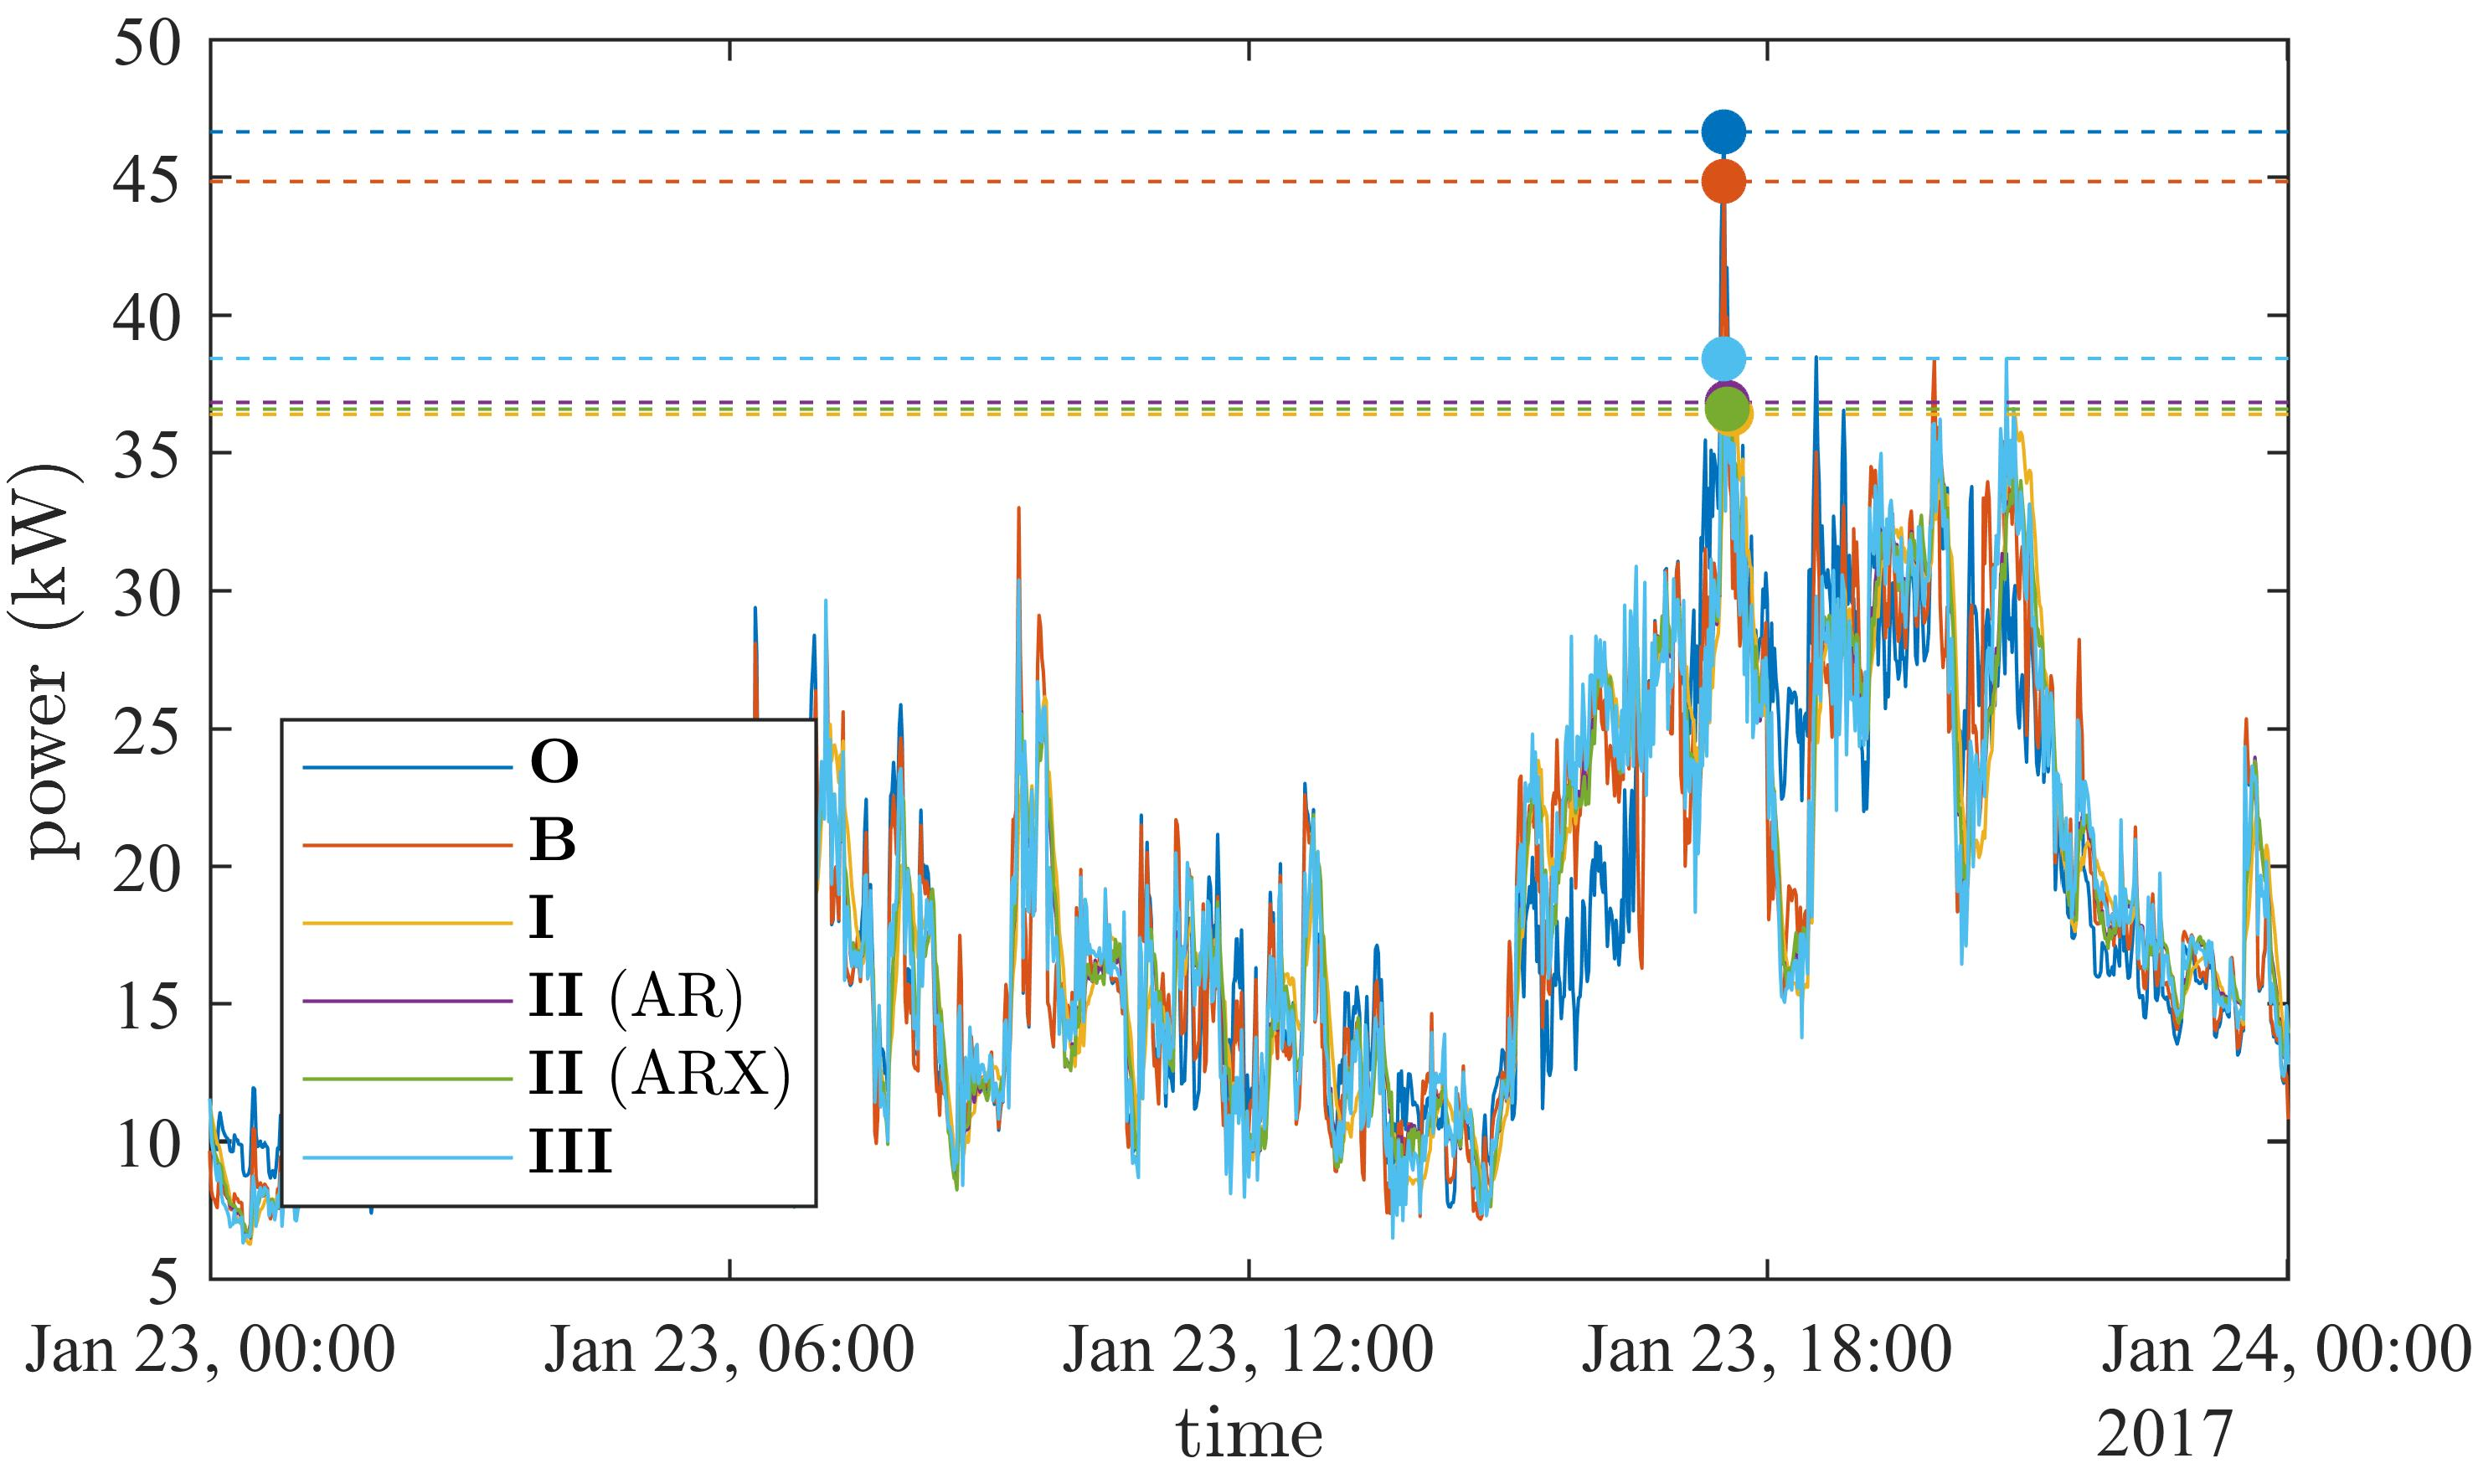
\includegraphics{_chapter2/fig/day-peak-1}
		\label{ch2:subfig:day-peak-total}
	}\\
	\subfloat[]{%
		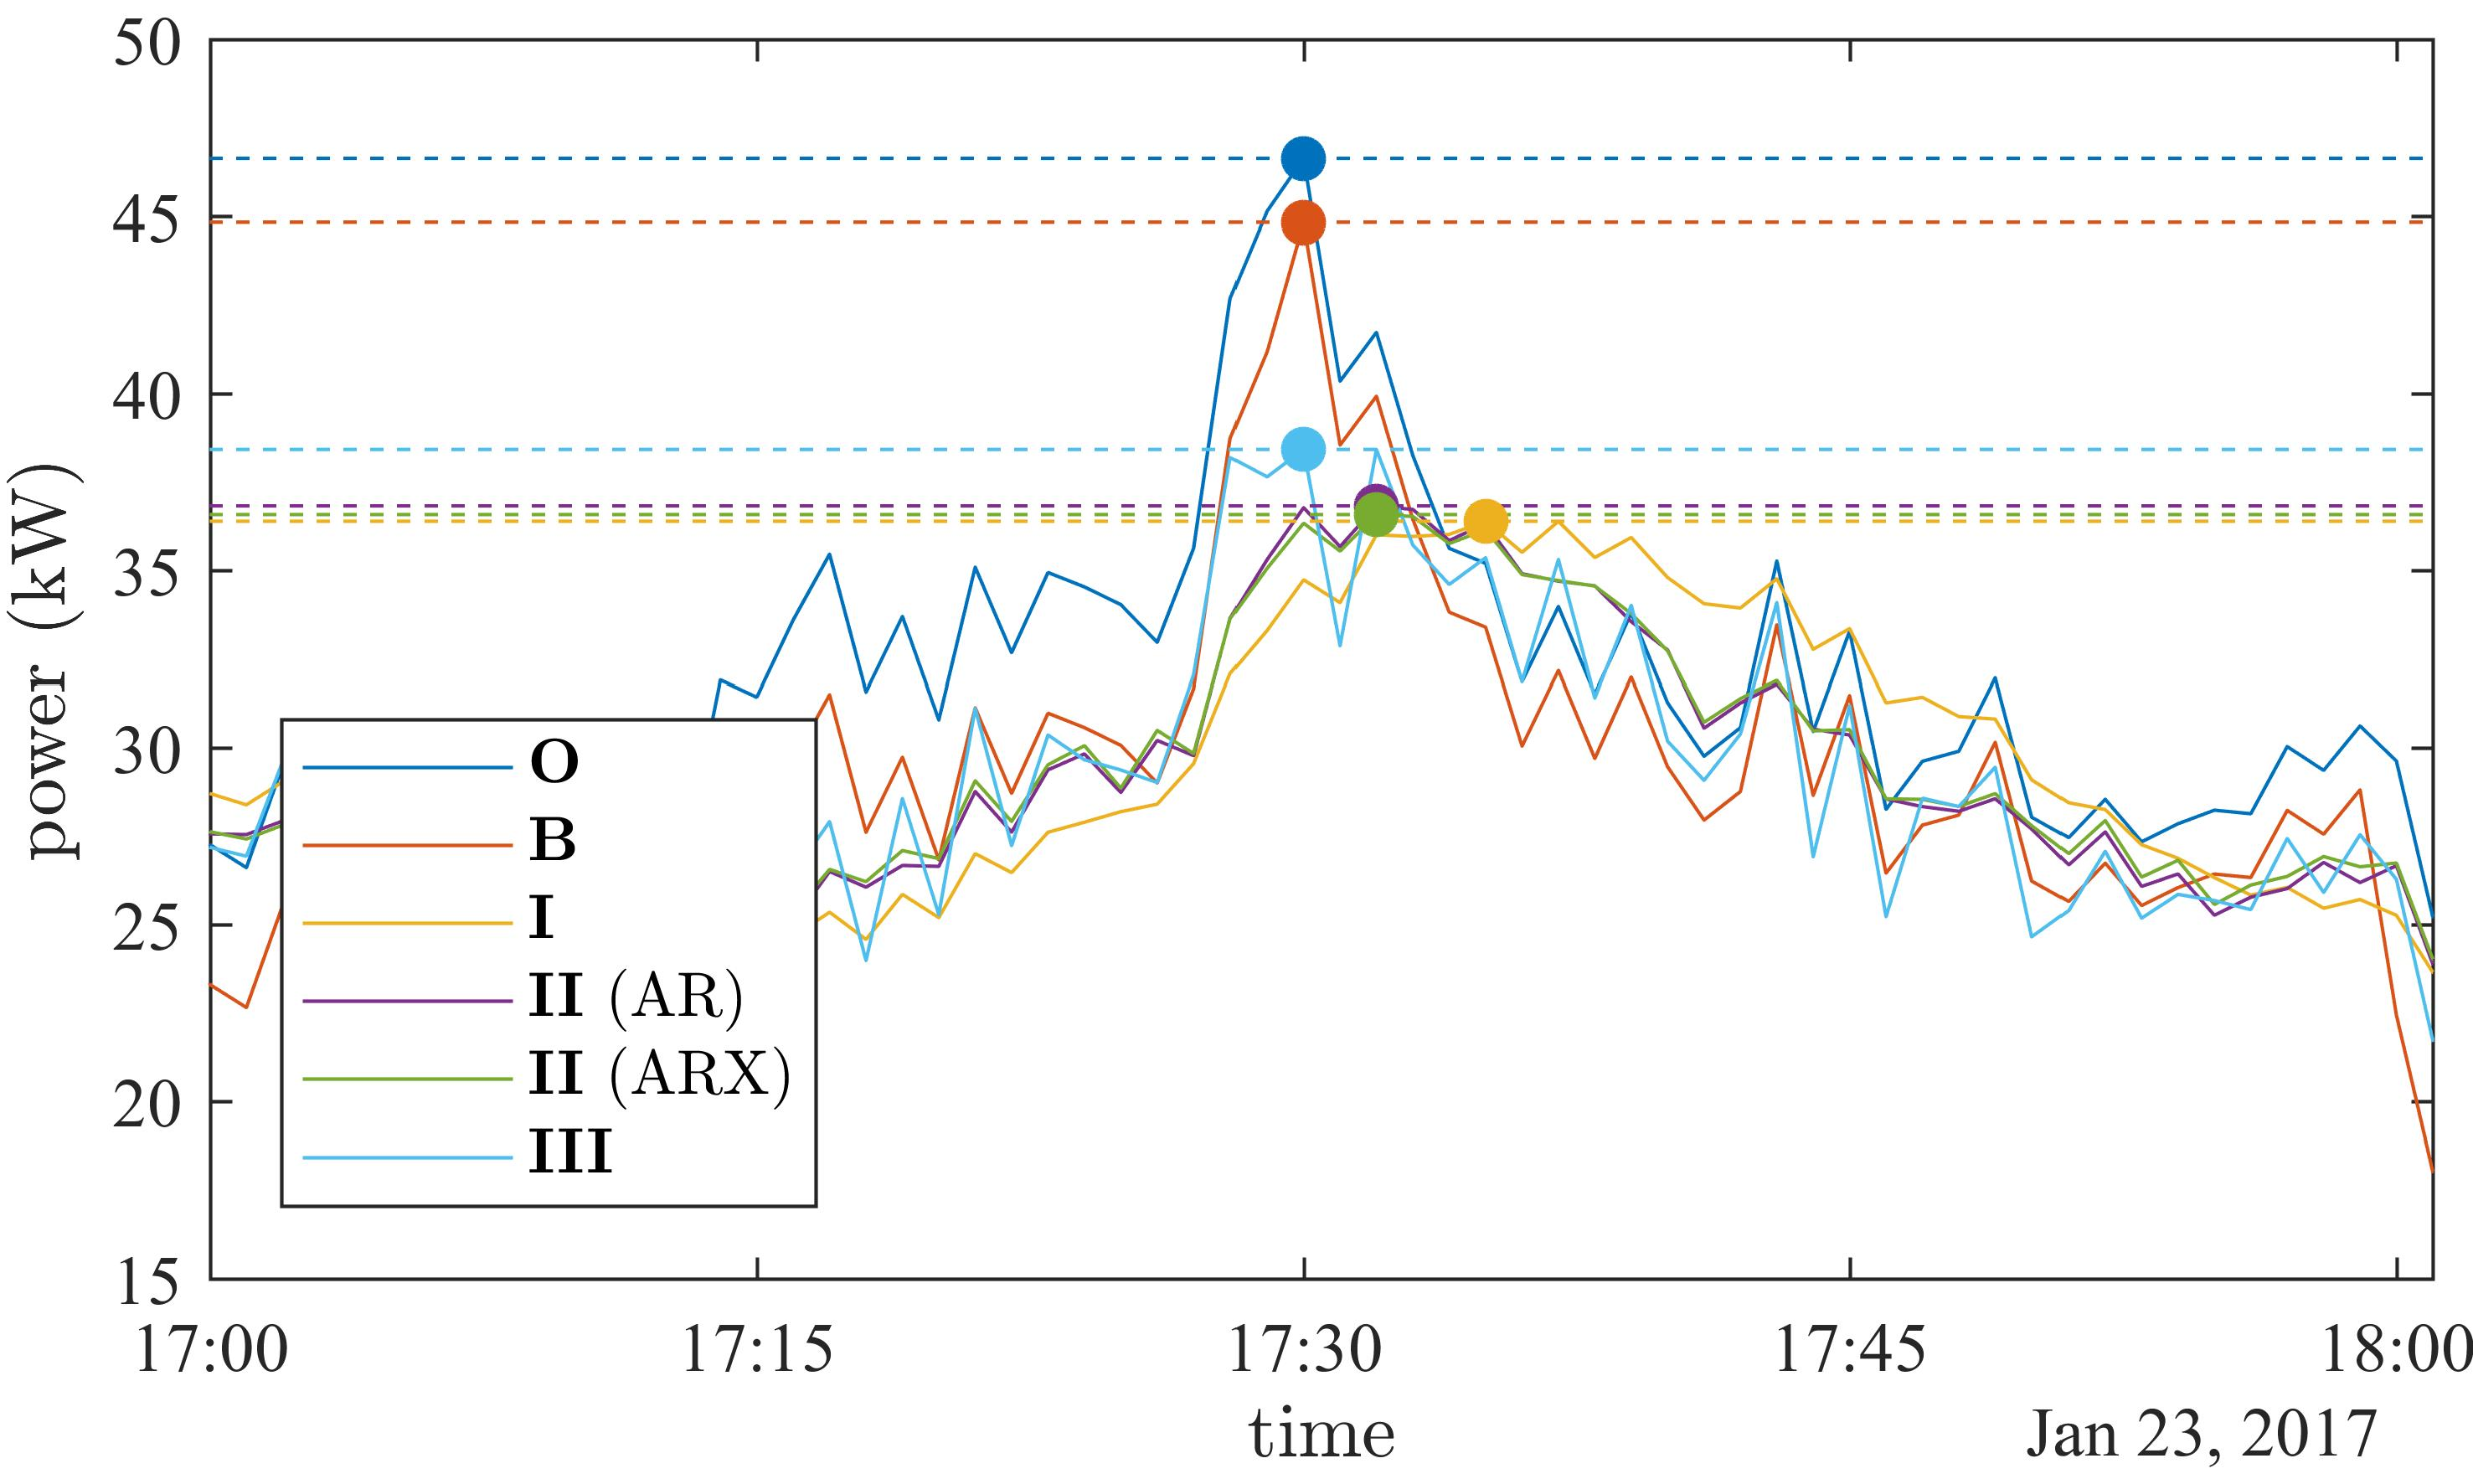
\includegraphics{_chapter2/fig/day-peak-1-zoom}
		\label{ch2:subfig:day-peak-zoomed}
	}
%	\subfloat[]{%
%		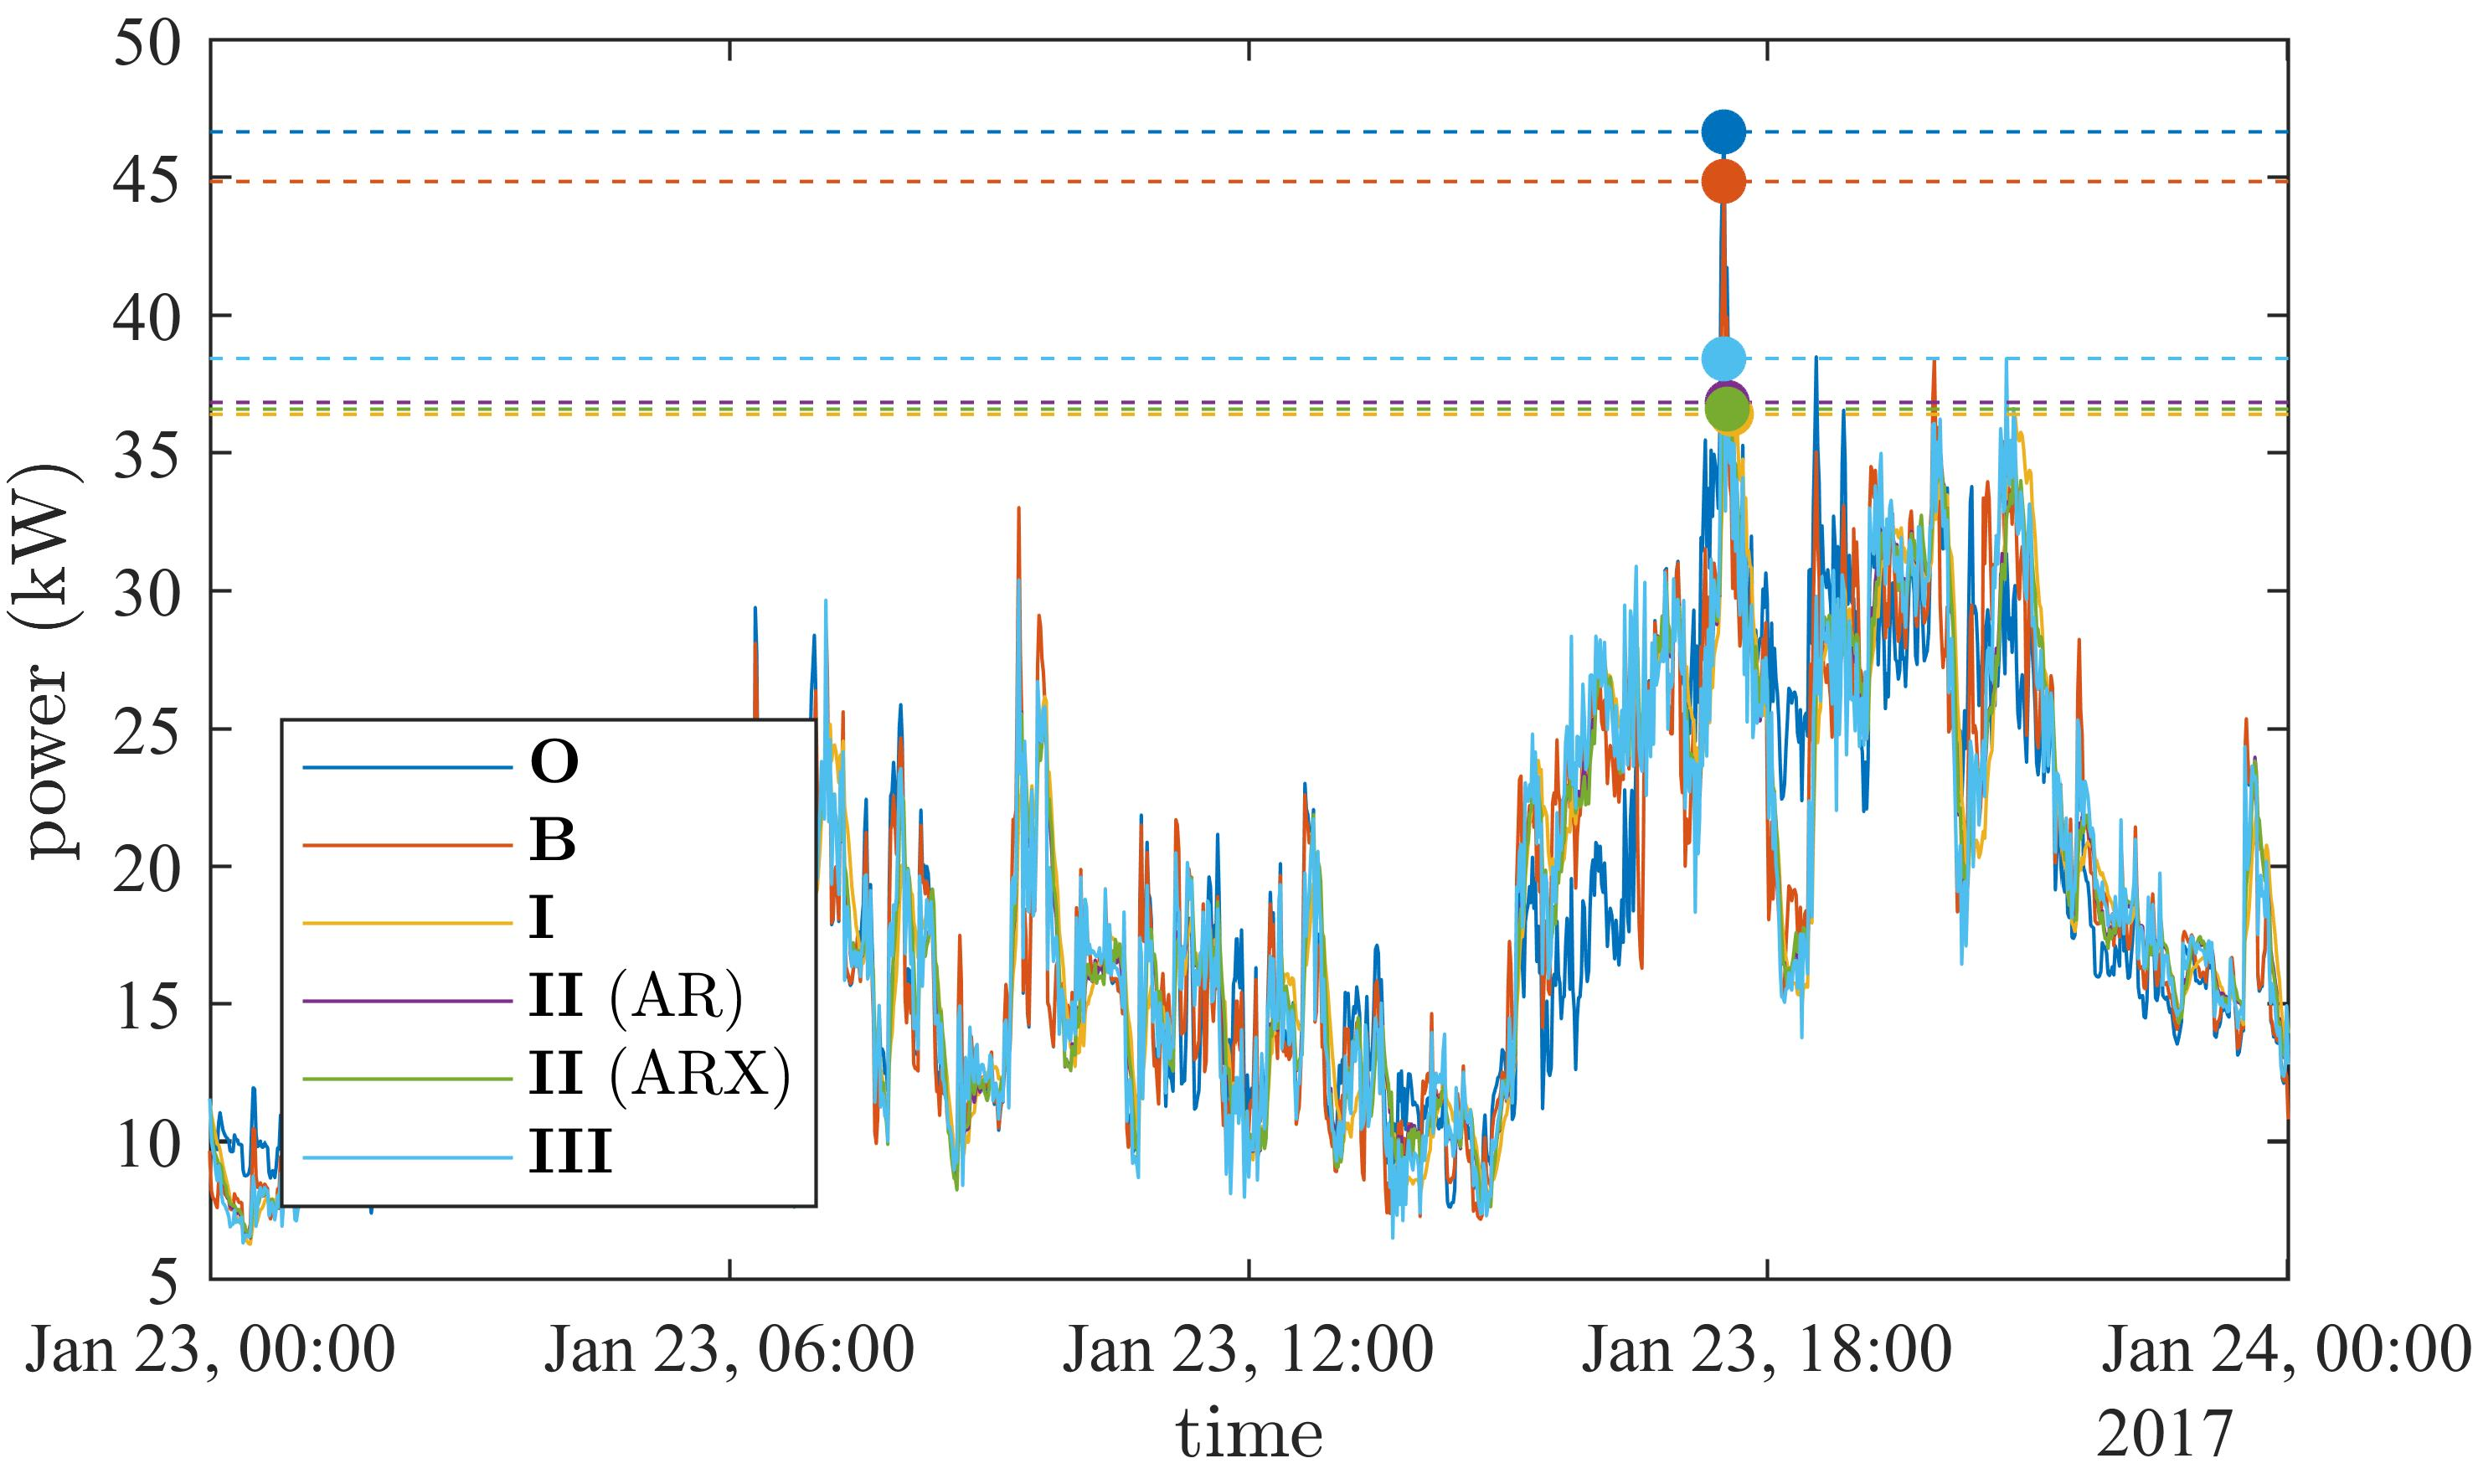
\includegraphics{_chapter2/fig/day-peak-1}
%		\label{ch2:subfig:day-peak-1}
%	}
%	\vspace{0mm}
%	\subfloat[]{%
%		\includegraphics{_chapter2/fig/day-peak-2}
%		\label{ch2:subfig:day-peak-2}
%	}
	\caption{Time series performance over a single day when using realistic load forecasts (total day in Figure \ref{ch2:subfig:day-peak-total}, and zoomed in on critical period in Figure \ref{ch2:subfig:day-peak-zoomed}).}
	\label{ch2:fig:day-peak}
\end{figure}

A single day was plotted in Figure~\ref{ch2:fig:day-peak} which shows the time-series improvements that were yielded by the ESMU operation.
For visual clarity Figure~\ref{ch2:subfig:day-peak-total} and \ref{ch2:subfig:day-peak-zoomed} show, respectively, the entire day and a zoomed in version that focuses on the period of interest where the ESMU impact is most apparent.
It can be observed that the unmodified demand profile (i.e. the original case  \textbf{O}) and the case where scheduled half-hourly ESMU operation is applied (i.e. the  baseline case \textbf{B}) result in noticeably higher load peaks than any of the three adjustment cases.
More specifically, the original peak reduction (which is equal to the scheduled ESMU power) was 1.8kW (or 3.9\% peak reduction).
The average peak reduction when applying adjustments to the ESMU operation was 9.6kW (or 20.6\% peak reduction).
Although it is too early to conclude on any overall performance improvements this time-series modification does show the physical impact of the ESMU schedule adjustments on the network's load profile.
Furthermore Figure~\ref{ch2:subfig:day-peak-total} highlights the volatility of the underlying data which would be neglected for half-hourly ESMU schedules.

Interestingly, both the standard AR and the exogenous AR estimation models that were used in case \textbf{II} performed very similar and show little to no significant difference in peak reduction performance.
Equally noteworthy is the fact that the simplest prediction methods of them all in case \textbf{III} (i.e. the method of assuming a power repetition occurs) yields positive peak power reductions, too.
However, case \textbf{I} slightly outperformed all other cases since perfect knowledge would also imply best results.
Nonetheless, only a small improvement was possible due to the imperfect underlying half-hourly ESMU schedule.
The amount by which the three cases were able to reduce the daily peak load is also indicated by horizontal dashed lines and dots located at the point of peak load for each profile.
These initial findings show that every single version of dynamic control reduces peak load when compared to the baseline case \textbf{B}.
This finding is also tabulated in Table~\ref{ch2:tab:ts-table}, and it suggests that the prediction mechanism by itself did play some role when compensating for demand volatility.

\begin{table}\centering
%	\begin{tabular}{r | c}
%		case & peak load\\% & ideal forecast\\
%		\hline
%		\textbf{O} & 46.6kW\\
%		\textbf{B} & 44.8kW\\
%		\textbf{I} & 36.4kW\\% & \textbf{IV}\\
%		\textbf{II} (AR) & 36.8kW\\% & \textbf{V}\\
%		\textbf{II} (ARX) & 36.6kW\\% & \textbf{V}\\
%		\textbf{III} & 38.4kW\\% & \textbf{VI}\\
%	\end{tabular}
	\begin{tabular}{r | c | c | c | c | c | c}
		\multirow{2}{*}{case} & \multirow{2}{*}{\textbf{O}} & \multirow{2}{*}{\textbf{B}} & \multirow{2}{*}{\textbf{I}} & \textbf{II} & \textbf{II} & \multirow{2}{*}{\textbf{III}}\\% & ideal forecast\\
		& & & & \tiny{(AR)} & \tiny{(ARX)} & \\% & ideal forecast\\
		\hline
		peak & \multirow{2}{*}{46.6} & \multirow{2}{*}{44.8} & \multirow{2}{*}{36.4} & \multirow{2}{*}{36.8} & \multirow{2}{*}{36.6} & \multirow{2}{*}{38.4}\\
		(kW) & & & & & & \\
	\end{tabular}
	\caption{Peak reduction in time-series sample}
	\label{ch2:tab:ts-table}	
\end{table}

However, the general impact of each prediction method on the resulting peak reduction performance can only be assessed if the complete dataset is evaluated.
Hence, the next section compares the daily peak load reduction from the application of each case.

\subsection{Daily peak reduction}

\begin{figure}\centering
	\subfloat[]{%
		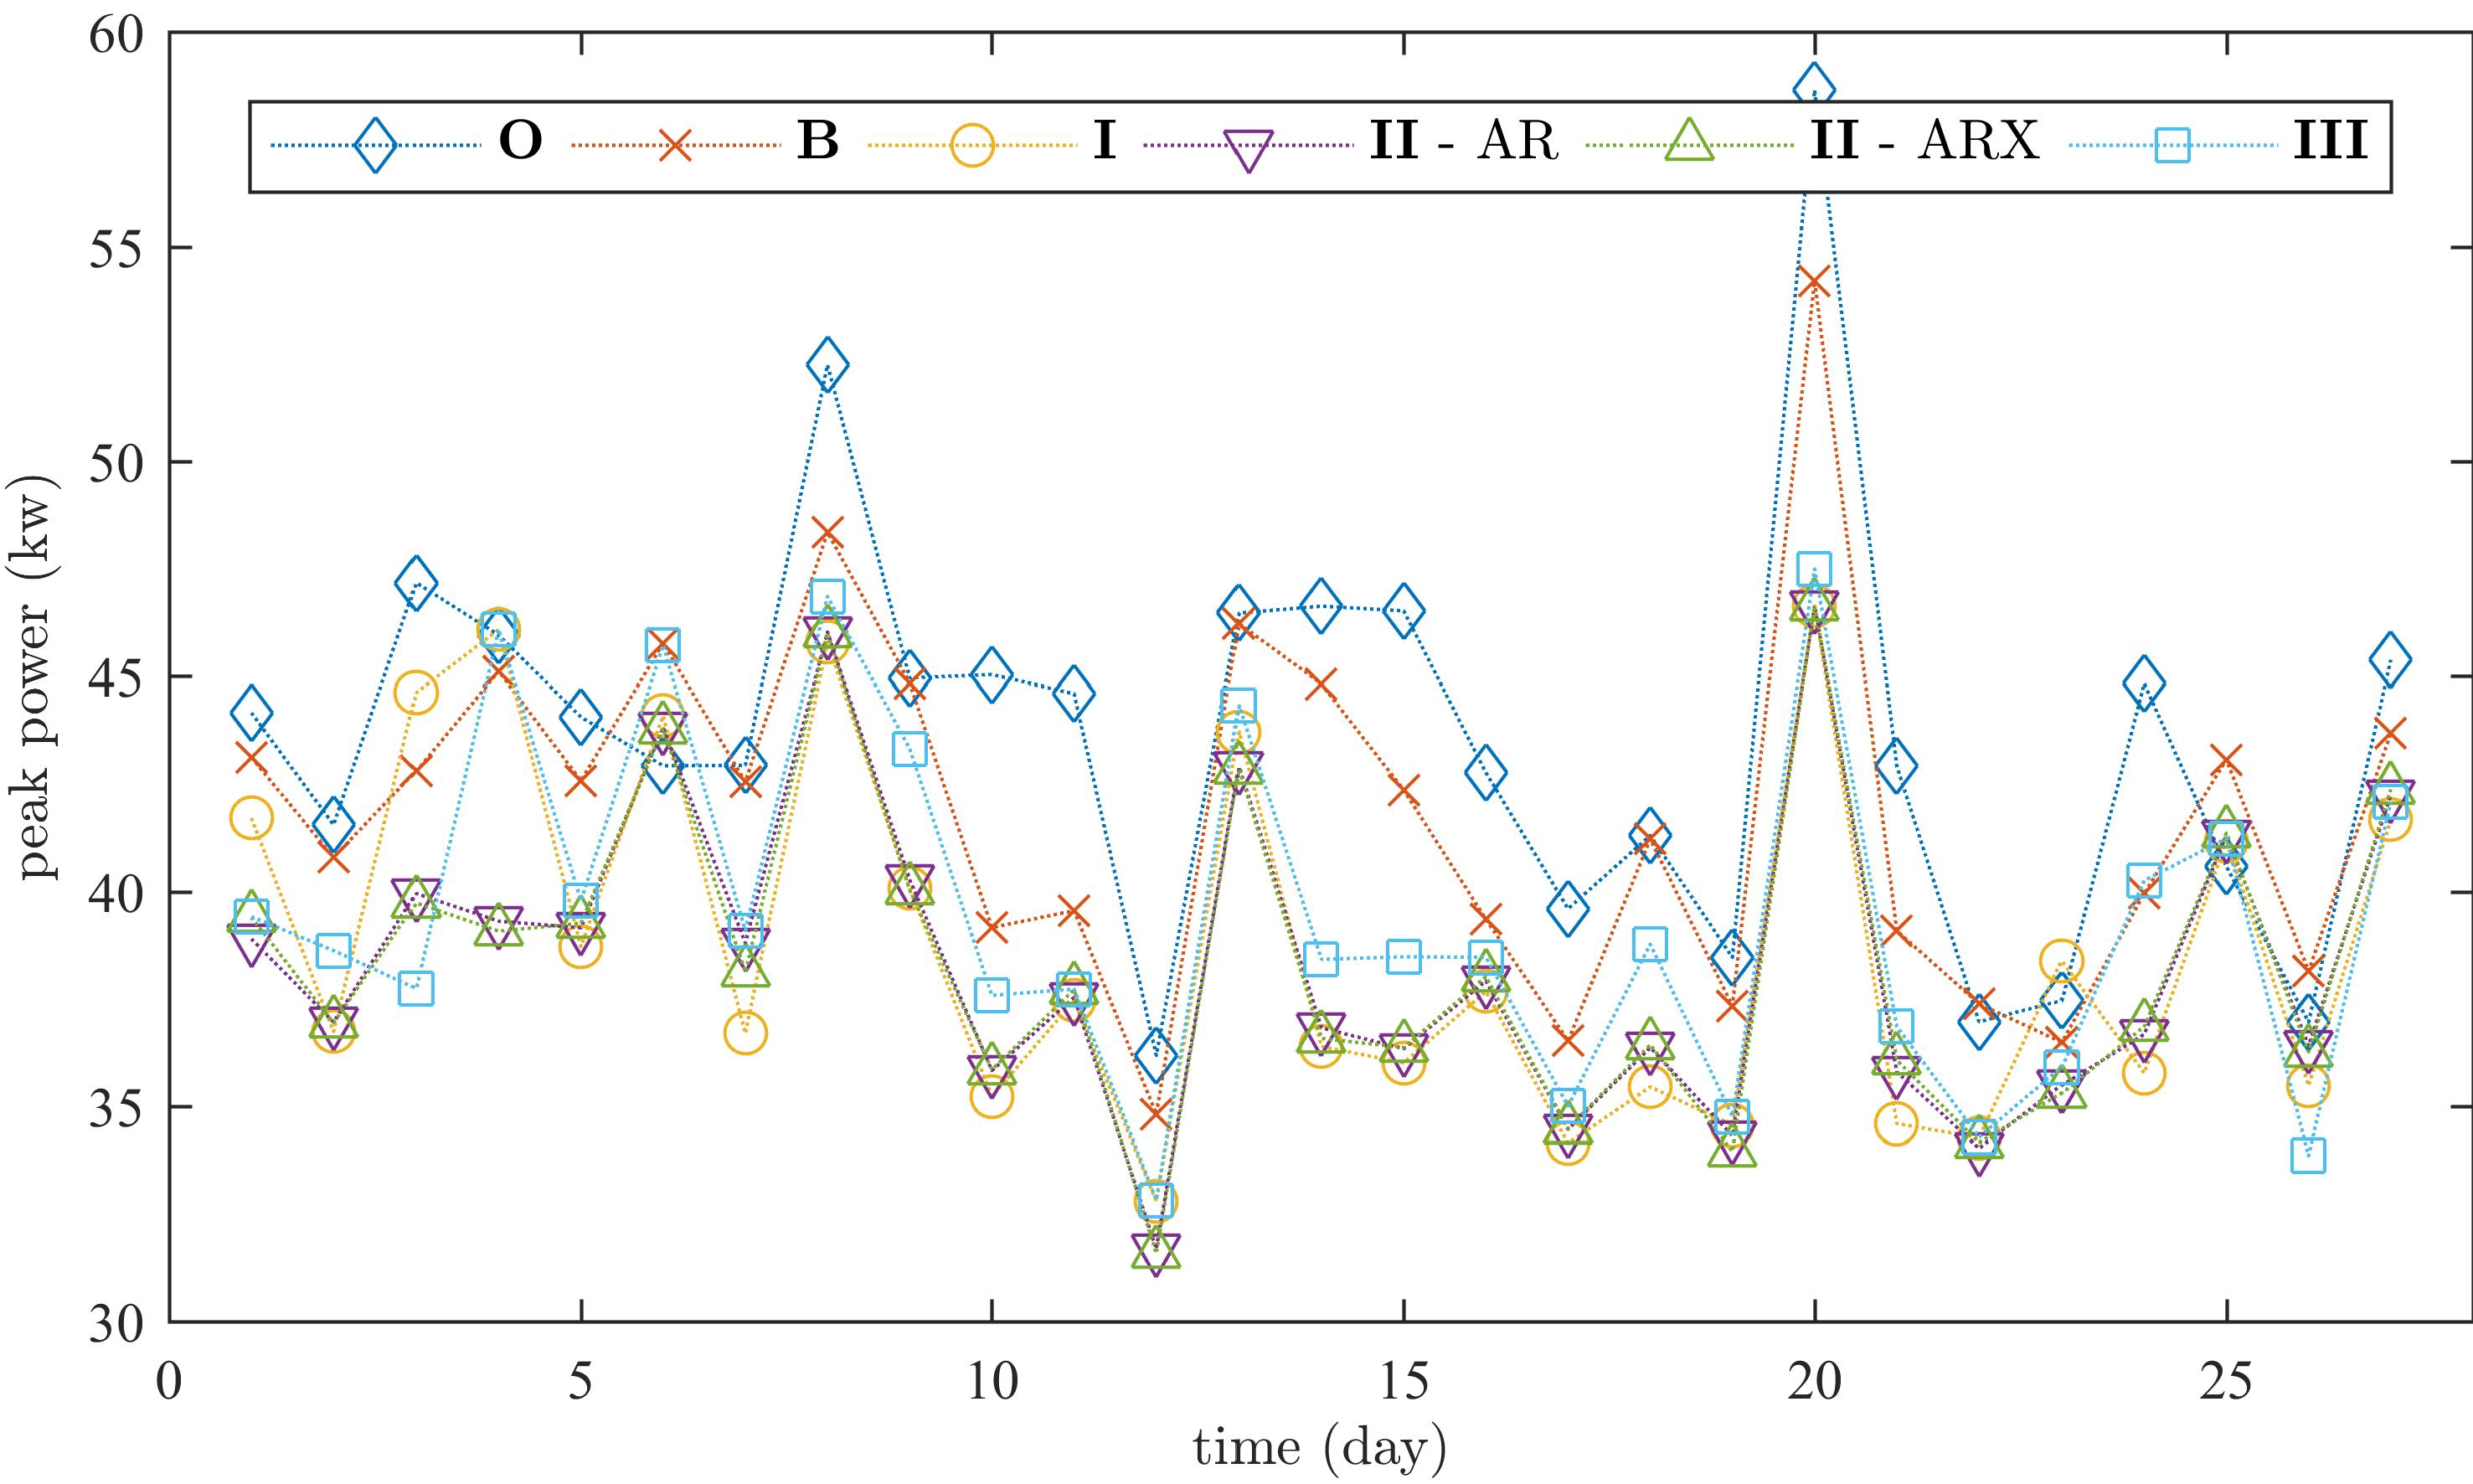
\includegraphics{_chapter2/fig/daily-peaks-1}
		\label{ch2:subfig:daily-peaks}
	}\\
	\subfloat[]{%
		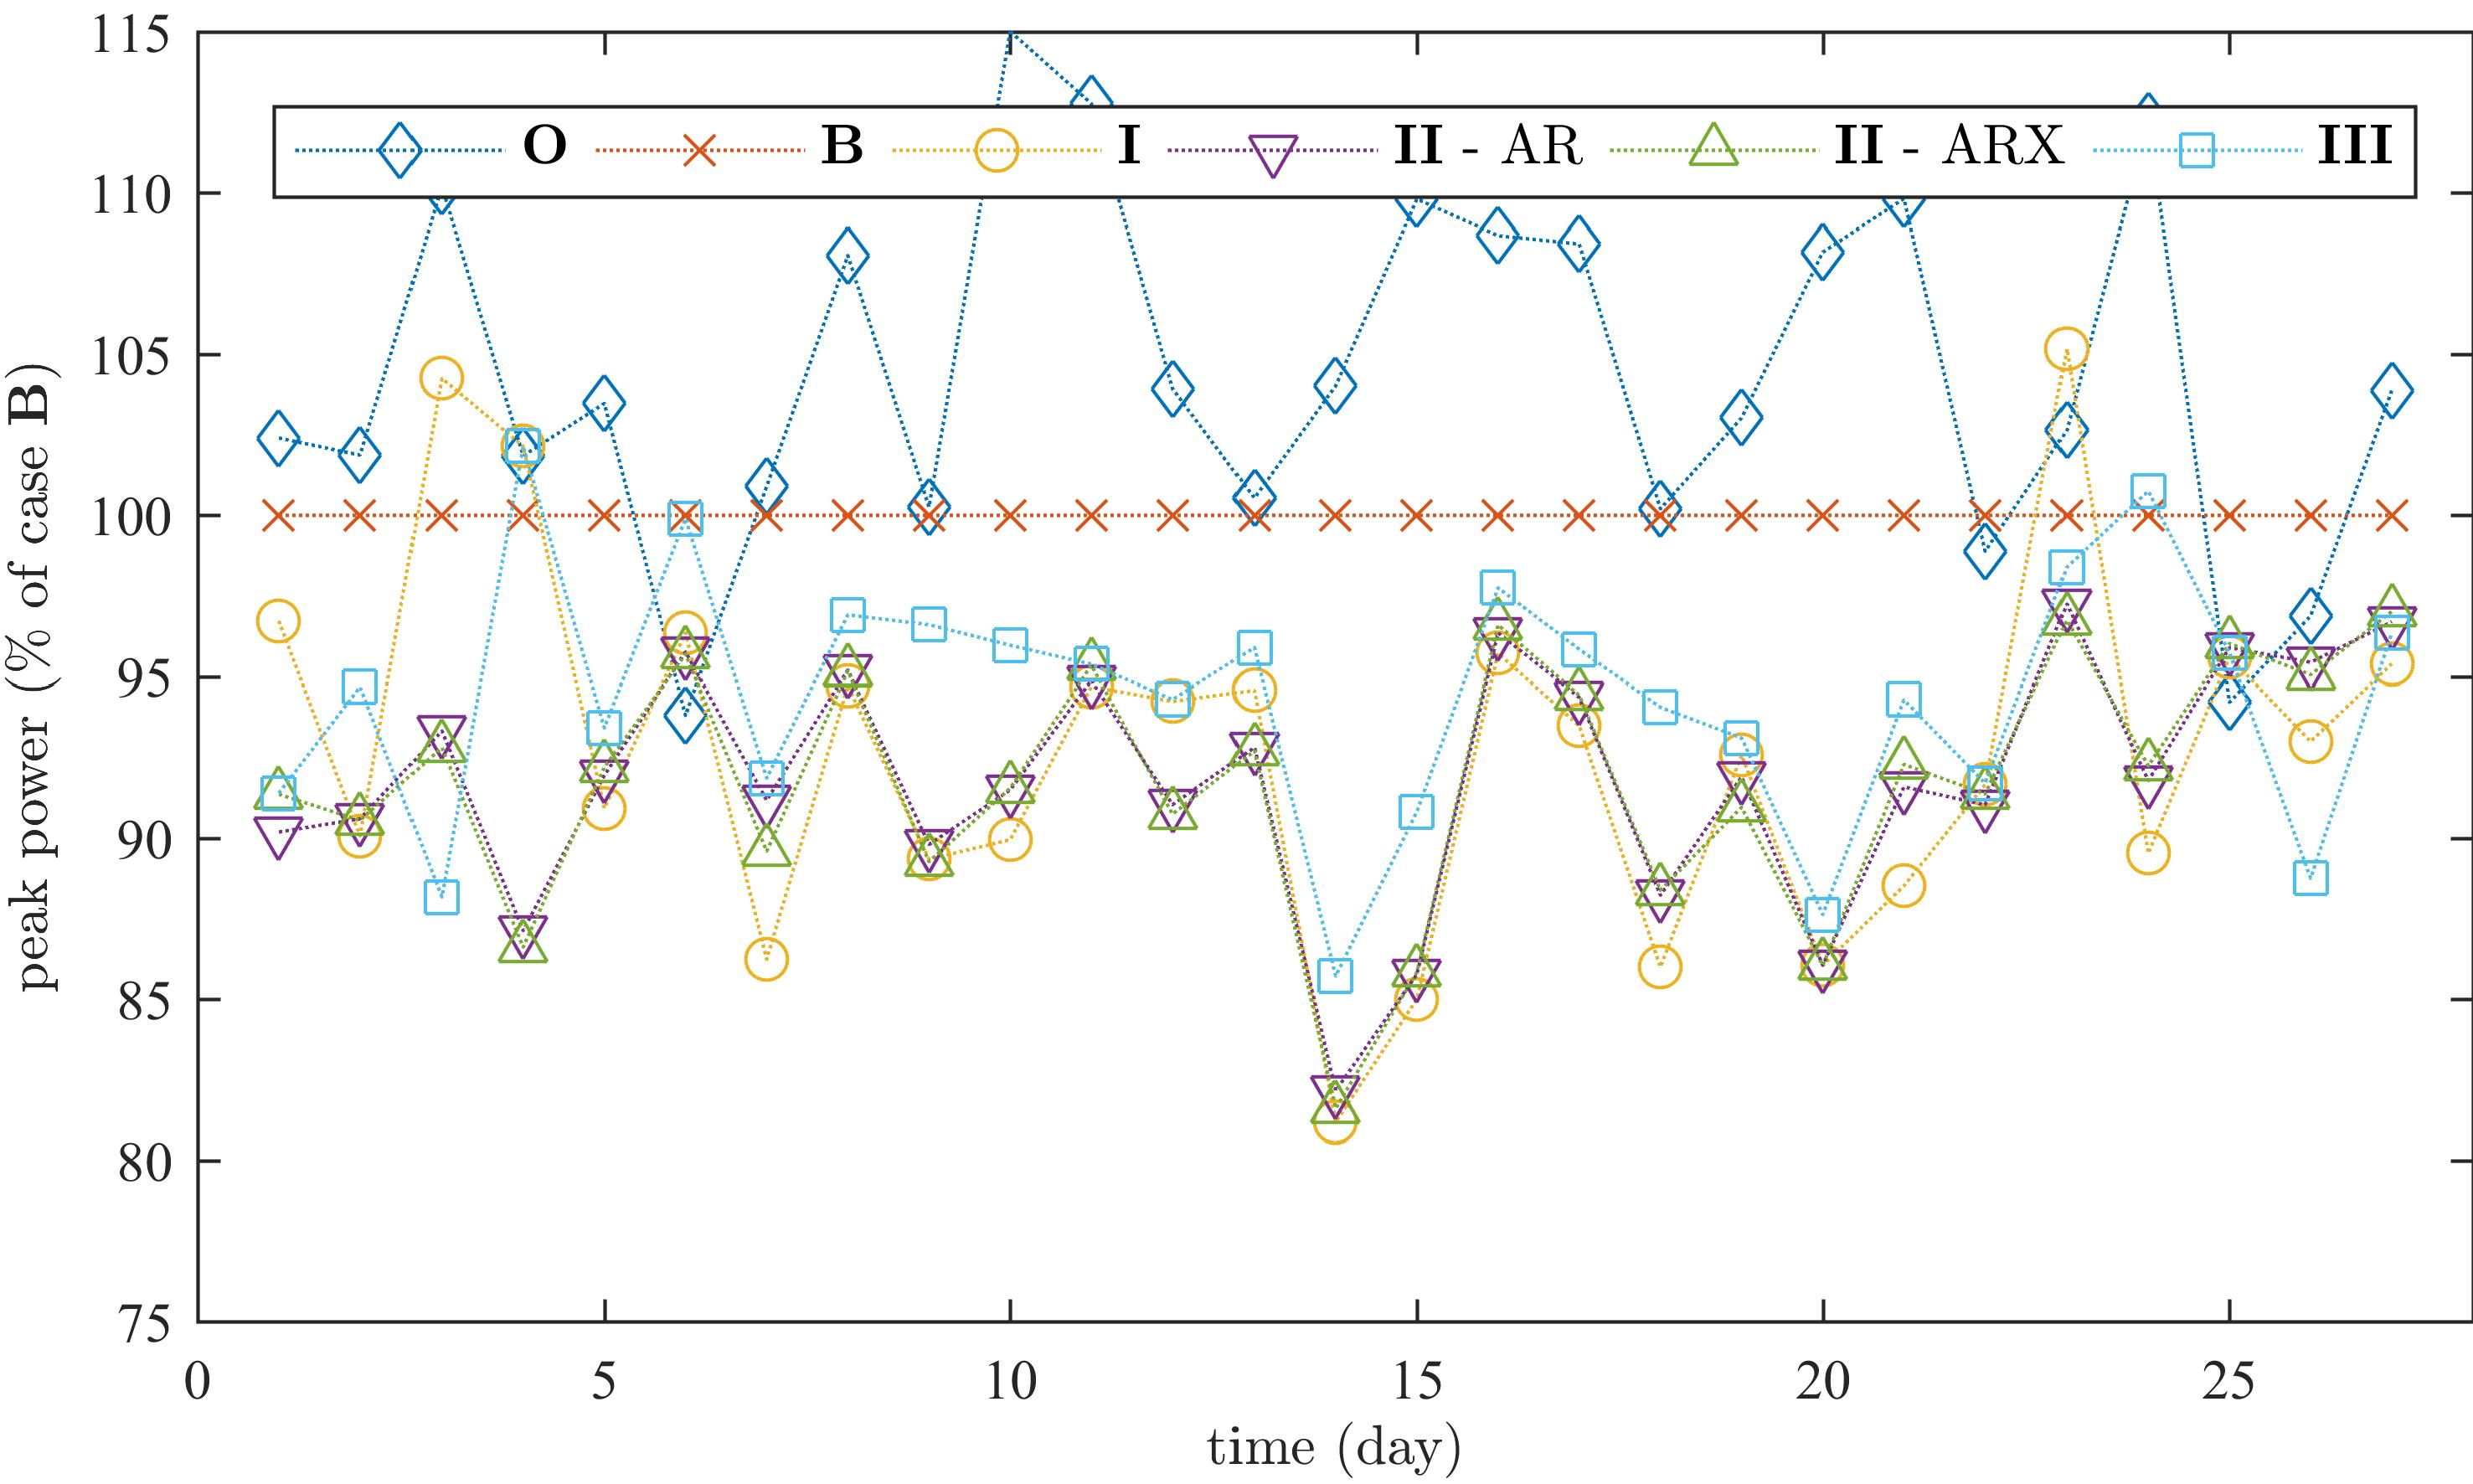
\includegraphics{_chapter2/fig/daily-peaks-1-percentage}
		\label{ch2:subfig:daily-peaks-percentage}
	}
	\caption{Daily peak reduction when using realistic forecasts as: (\ref{ch2:subfig:daily-peaks}) peak power values; (\ref{ch2:subfig:daily-peaks-percentage}) percentage of original case \textbf{B}.}
	\label{ch2:fig:daily-peaks}
\end{figure}

In Figure~\ref{ch2:fig:daily-peaks}, every day's power peak was extracted in a similar way to the procedure that was used for Figure~\ref{ch2:fig:day-peak}.
Here the actual power peaks were plotted in Figure~\ref{ch2:subfig:daily-peaks}, and the relative power improvements (i.e. ratio to the baseline power peaks from case \textbf{B}) were plotted in Figure~\ref{ch2:subfig:daily-peaks-percentage}.
From both plots it can be seen that controlling ESMU using the proposed dynamic control \hladd{(\textbf{I}, \textbf{II}, \textbf{III}) }lowers peak load.
This is true even when the underlying ESMU schedule originally worsened and increased peak load\hladd{ (see \textbf{B} vs \textbf{O})}.
Such a behaviour can be observed clearly during \hlrem{e.g.} days 6 and 25, where the half-hourly ESMU schedule\hladd{ based on \textbf{B}} increased the actual load peak\hladd{ from case \textbf{O}} by 2.8kW and 2.5kW, respectively.
The ESMU schedule adjustment mechanisms \hladd{(\textbf{I}, \textbf{II}, \textbf{III}) }however compensated for this error, but in those two cases the compensation was not enough to reduce peak power below the original value.
Day 26 on the other hand experienced a similar increase in peak power during the baseline case \hlrem{(i.e. case }\textbf{B}\hlrem{)} by 1.2kW, but the \hladd{proposed }power adjustment mechanism \hladd{according to \textbf{II}}corrected this forecast error and reduced the final peak power below the original value.

Nonetheless, the sensitivity to the underlying power prediction approaches becomes apparent when having this larger set of peak reduction results to compare the dynamic control's performance against its baseline cases.
As seen in Figure~\ref{ch2:subfig:daily-peaks-percentage} the scenario with perfect foresight (i.e. case \textbf{I}) frequently outperformed all other cases since it appears to achieve largest peak power reduction from the baseline case.
During some days however (i.e. day 3, 4 and 24) the compensators could not correctly compensate despite the perfect foresight.
This behaviour was unexpected, but it turns out that the discrepancy between the underlying half-hourly BESS schedule and the actual load curve (i.e. due to erroneous half-hourly load forecasts) caused the dynamic control to reach its SOC tolerance limit.
Reaching its limit during those three days consequently worsened the daily peak.
The simplest of all cases on the other hand (i.e. case \textbf{III}) yielded a constant but small reduction when compared to the baseline case.
Case \textbf{II} seems to perform similar, but slightly better than case \textbf{III}.
One could therefore assume that by maintaining a constant error in the power prediction does positively skew the results when already subjected to low-resolution forecasting errors.
Whether this assumption holds can however not be said with the presented analysis and instead, in order to obtain an more general picture of the overall peak reduction performance, the Probability Density Function (PDF) had to be estimated and analysed for all cases.
This is done in the following section.

\subsection{Probability of peak reduction}
\label{ch2:subsec:probability-of-peak-reduction}

\begin{figure}\centering
	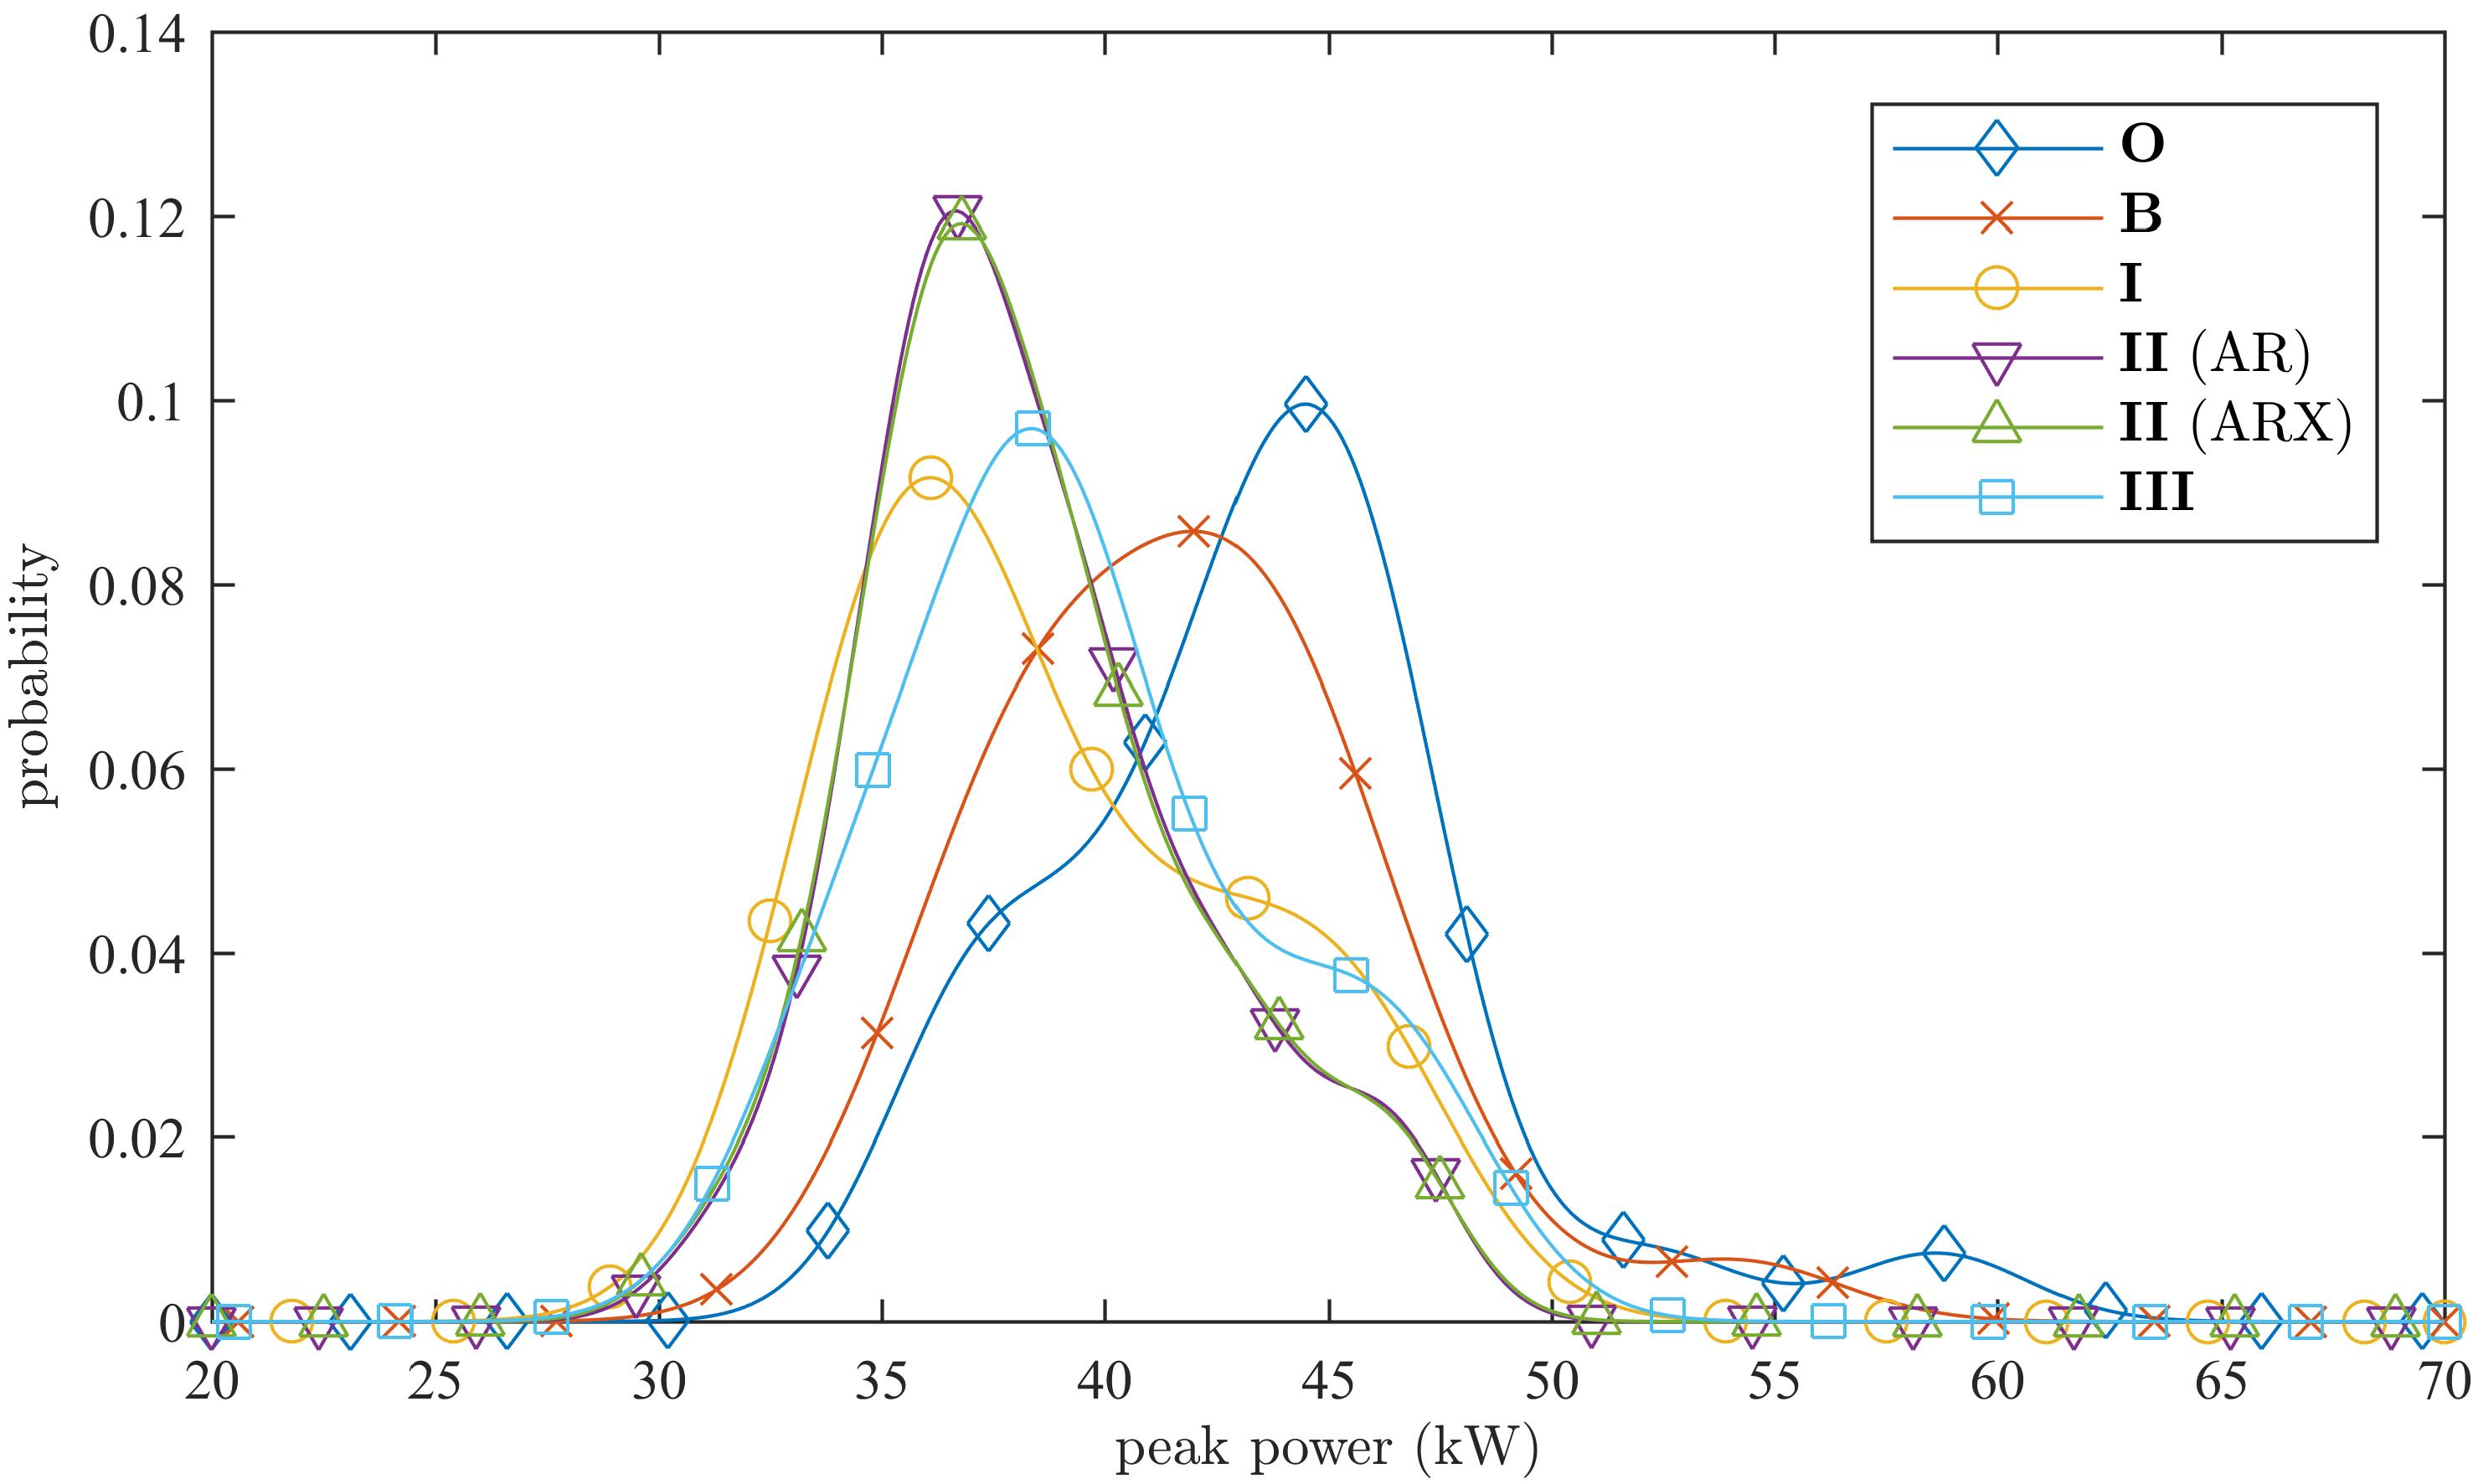
\includegraphics{_chapter2/fig/pdf-1-avg}
%	\subfloat[]{%
%		\includegraphics{_chapter2/fig/pdf-1}
%		\label{ch2:subfig:peak-pdf-1}
%	}
%	\vspace{0mm}
%	\subfloat[]{%
%		\includegraphics{_chapter2/fig/pdf-2}
%		\label{ch2:subfig:peak-pdf-2}
%	}
	\caption{Probability of load peak when using realistic forecasts.}
	\label{ch2:fig:peak-pdf}
\end{figure}

With the use of the standard kernel density estimation, the PDF is plotted in Figure~\ref{ch2:fig:peak-pdf}.
The data used to generate these plots is the same data as shown in Figure~\ref{ch2:fig:daily-peaks}.
Now however, the probability of a peak power occurring is linked to the magnitude of this peak.
It can be seen that case \textbf{O} has the highest probability around a peak load of 45kW, whilst case \textbf{B} has its highest probability around a peak load of 42kW.
This indicates that there is even a high probability that the half-hourly ESMU schedule has a positive impact on the load peaks.
When adjusting this schedule by using the proposed dynamic control, this peak was however lowered further.
Case \textbf{I} performed best by having a most probable peak power of 36.1kW.
Case \textbf{II} achieve the second best values at 36.7kW and 36.8kW (for AR and ARX case, respectively) whilst the simplest prediction mechanism has its peak power probability maximised at 38.4kW.

\begin{figure}\centering
	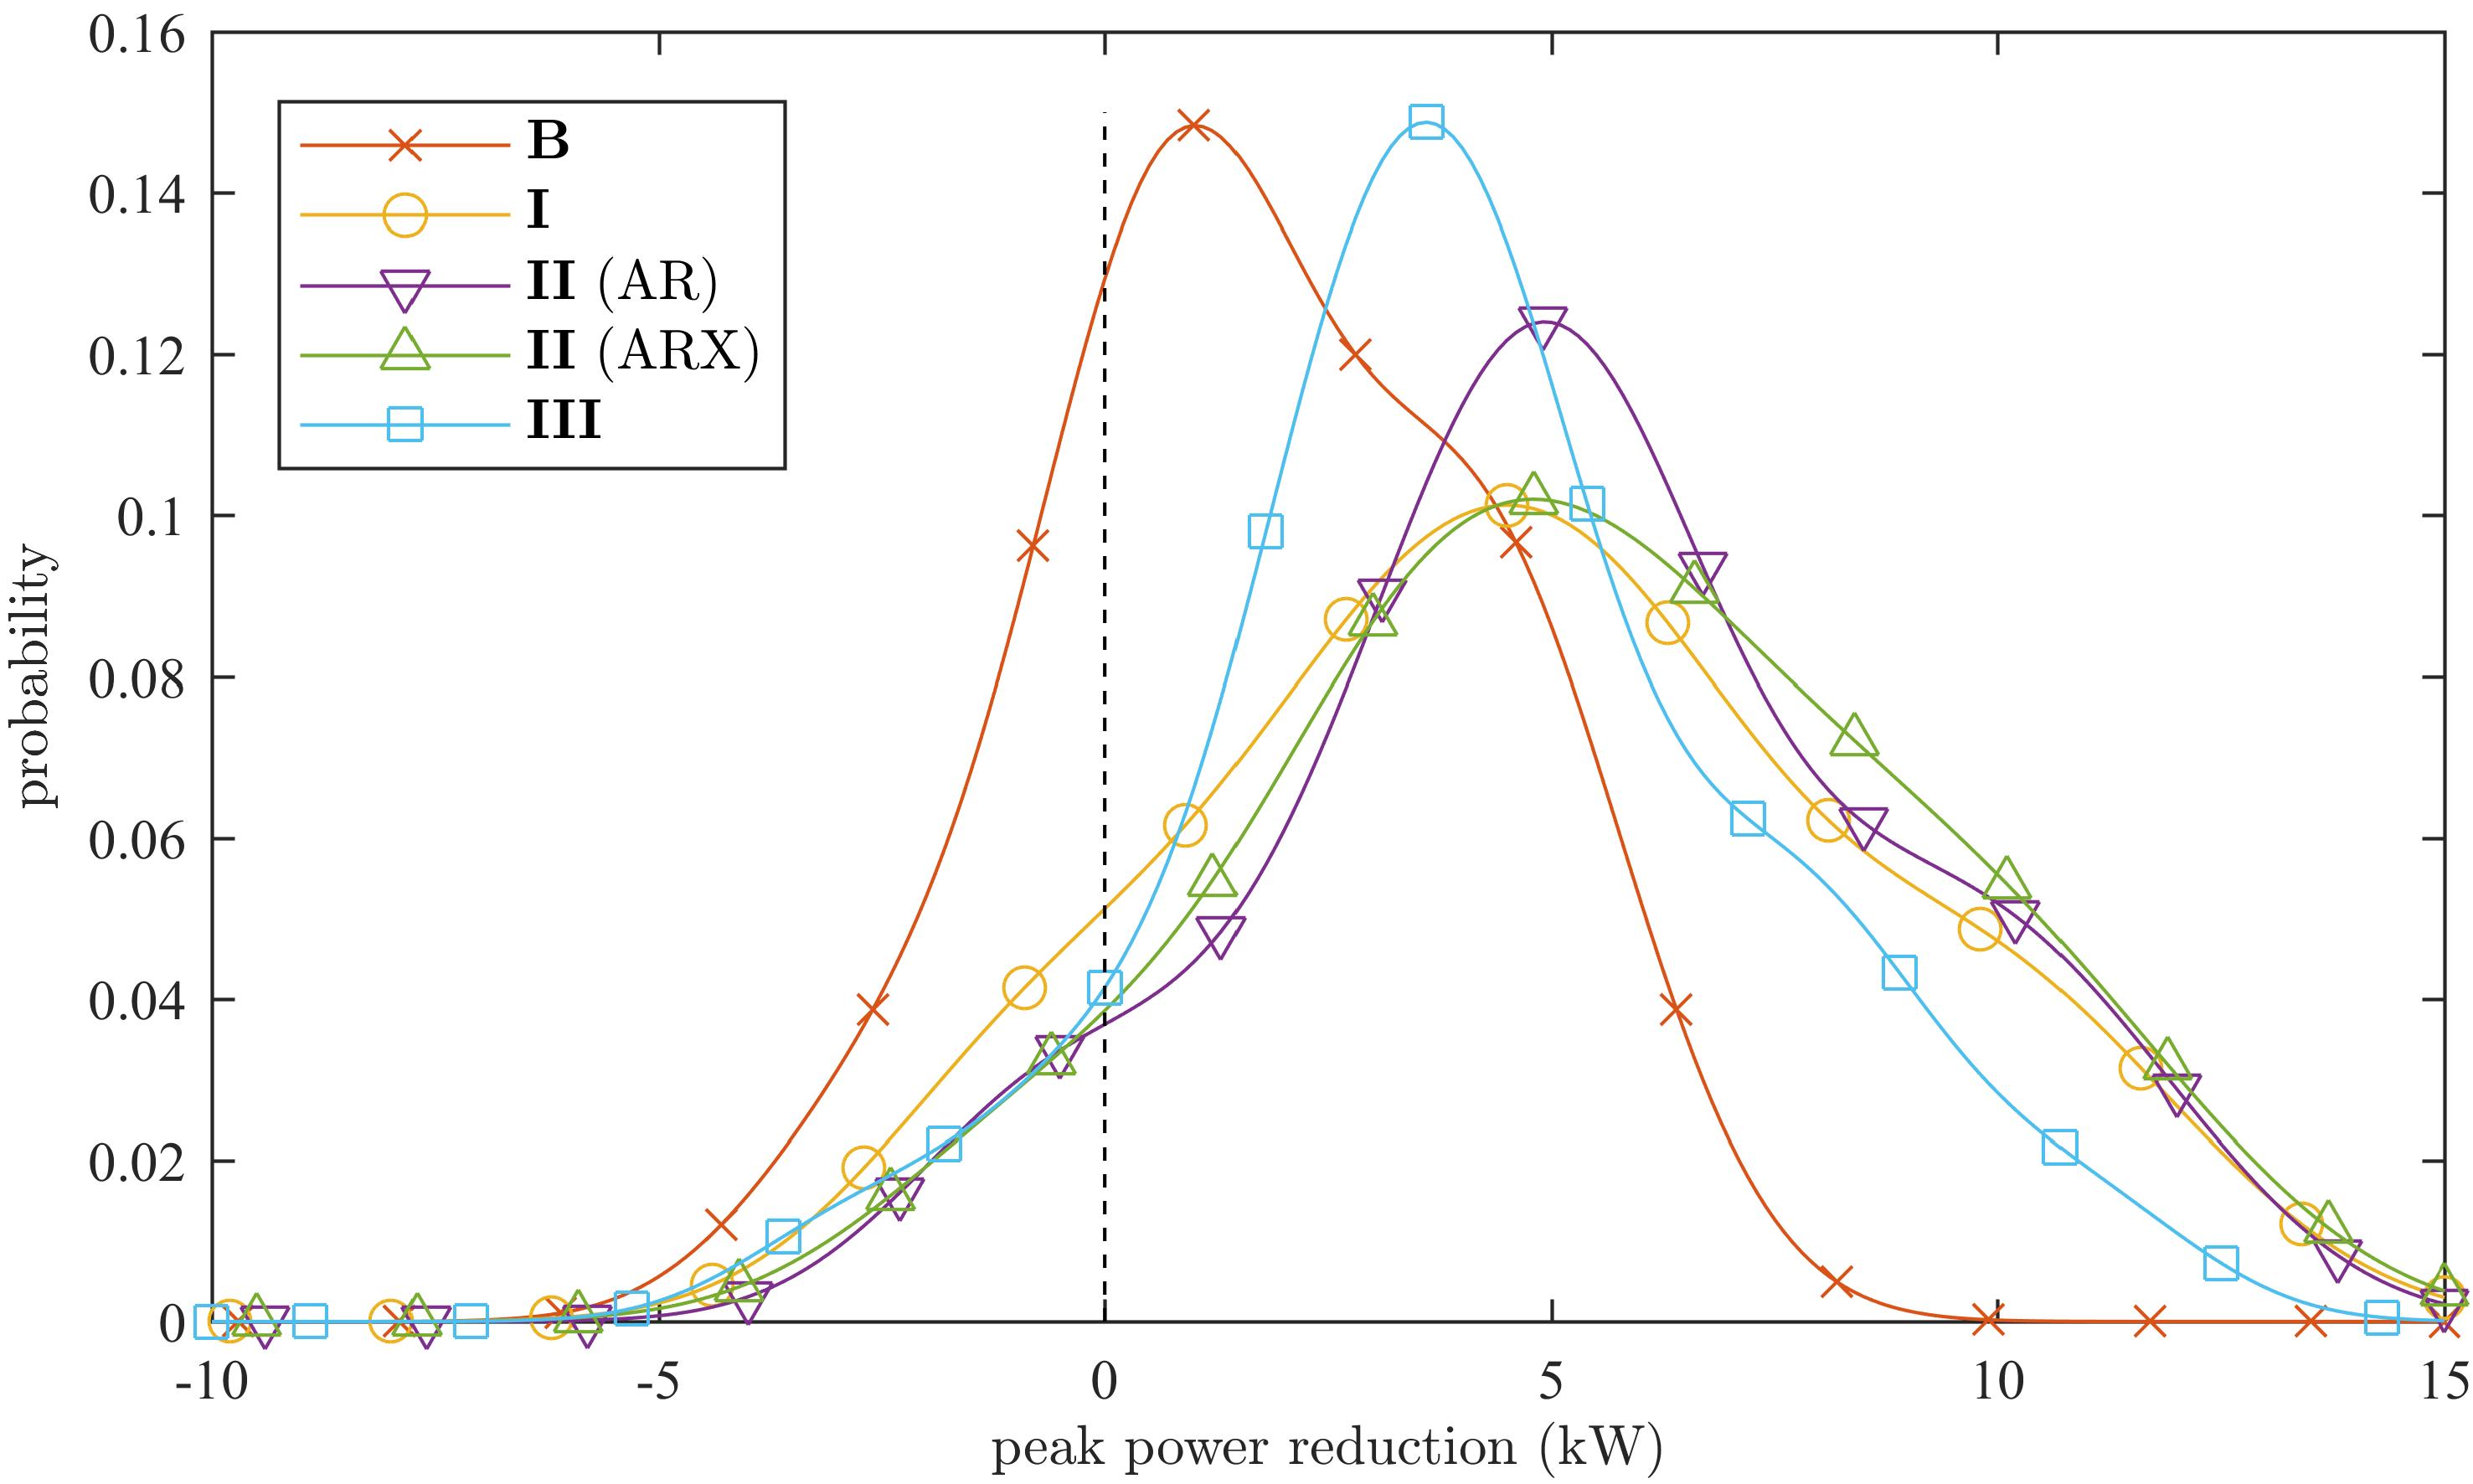
\includegraphics{_chapter2/fig/difference-pdf-1-avg}
%	\subfloat[]{%
%		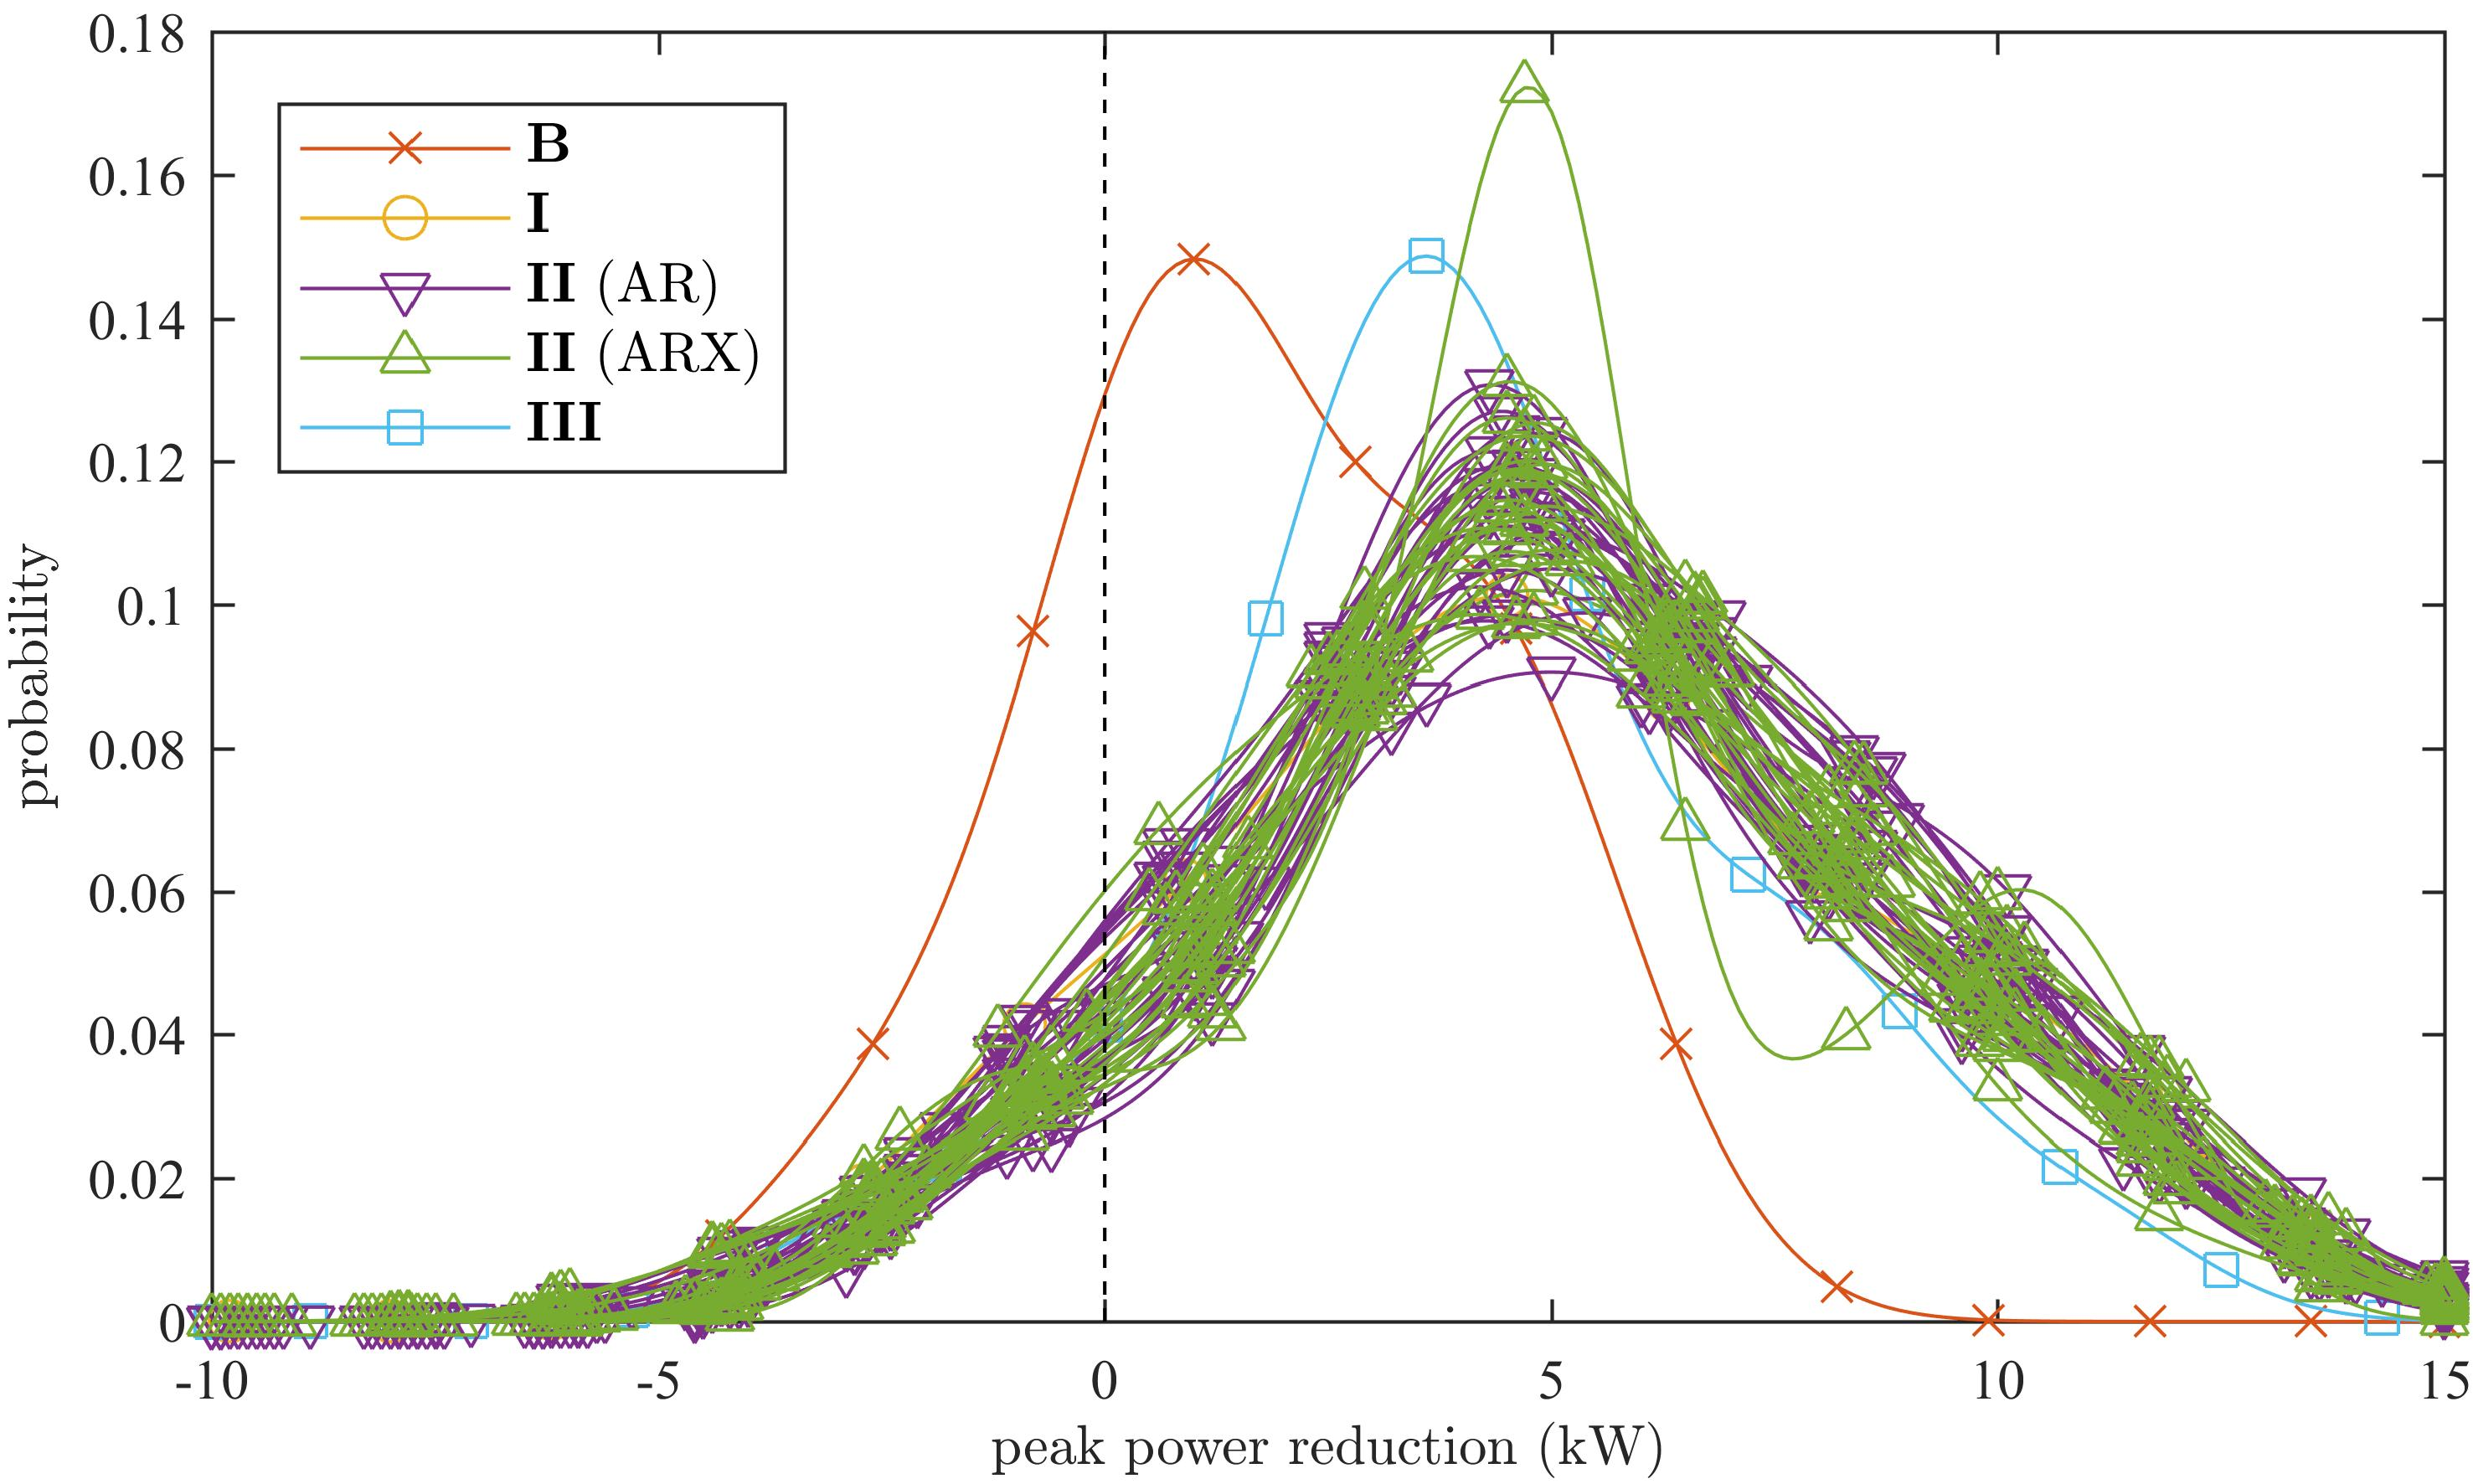
\includegraphics{_chapter2/fig/difference-pdf-1}
%		\label{ch2:subfig:peak-diff-pdf-1}
%	}
%	\vspace{0mm}
%	\subfloat[]{%
%		\includegraphics{_chapter2/fig/difference-pdf-2}
%		\label{ch2:subfig:peak-diff-pdf-2}
%	}
	\caption{Probability of load peak reduction when using realistic forecasts.}
	\label{ch2:fig:peak-diff-pdf}
\end{figure}

Figure~\ref{ch2:fig:peak-diff-pdf} takes this analysis even further where only the difference in peak load to the original case (i.e. case \textbf{O}) is plotted.
Now the ESMU impact can easily be seen since a high probability of positive peak load reduction indicates a beneficial impact of the ESMU operation.
A negative peak load reduction (i.e. increased peak load) would therefore indicate a worse performance.
As expected, case \textbf{B} has a slight positive impact on the system whilst a cumulative probability of more than 25\% (i.e. area under curve of case \textbf{O}) to the left of 0kW suggests that the peak might be worsened one in four times.
The dynamic control with its simplest prediction method however (i.e. case \textbf{III}) lowered this probability to already \hlrem{11.8\%}\hladd{7.4\%}.
The perfect foresight model (i.e. case \textbf{I}) performed \hlrem{best at} only \hlrem{7.4\%}\hladd{at 11.8\%} and the MPC based cases (i.e. case \textbf{II}) achieved an average of 8.0\% probability of worsening the peak power.
\hladd{The fact, that the perfect foresight model \textbf{III} could not reduce the probability of peaks as well as the simple model \textbf{I} is likely due to the used power profiles and forecast errors.
However, the mean probabilities (that are discussed below) differ as expected.}

\hladd{In the following, the mean peak reduction of the base case \textbf{B} (i.e. where the cumulative probability reaches 50\%) is treated as the benchmark for peak reduction.
This probability is reached at 1.7kW or in other words:}\hlrem{
Beside the reduced probability of missing or worsening peak load, the probability of having a larger positive impact is also increased when using the dynamic control.
Whilst} the probability of reducing load peaks by 1.7kW or more was at 50\% for case \textbf{B}\hladd{.
The}\hlrem{,} \hladd{simplest }case \textbf{III} \hladd{however }increased this probability to 77.7\%, case \textbf{II} to 84.5 5\% (AR) / 83.1\% (ARX), and the \hladd{perfect foresight }case \textbf{I} to 79.8\%.
The reason why this simplest case achieved a slightly lower value than the AR/ARX cases was due to aforementioned discrepancy between actual and forecasted load profiles.
Due to the discrepancy in erroneousness the chosen SOC tolerance was exhausted and lead to some worsening cases that negatively skewed results of the perfect foresight case (i.e. case \textbf{I}).
Nonetheless, when comparing the three dynamic control cases with each other as done in Figure~\ref{ch2:fig:peak-diff-pdf}, then it can be seen that case \textbf{II} using an AR model for MPC performed best at reducing peak loads for the used dataset.

\subsection{Impact of varying the model's length}

The subsequent results are intended to show whether the length of the AR/ARX model impacted the peak reduction performance.
To do so, the same procedure was use as shown in Section~\ref{ch2:subsec:probability-of-peak-reduction}, but the length of the AR and ARX models was varied from five minutes to two hours.
Therefore the MPC of the dynamic control took into account a longer power history to potentially improve the prediction of the next power.

\begin{figure}\centering
	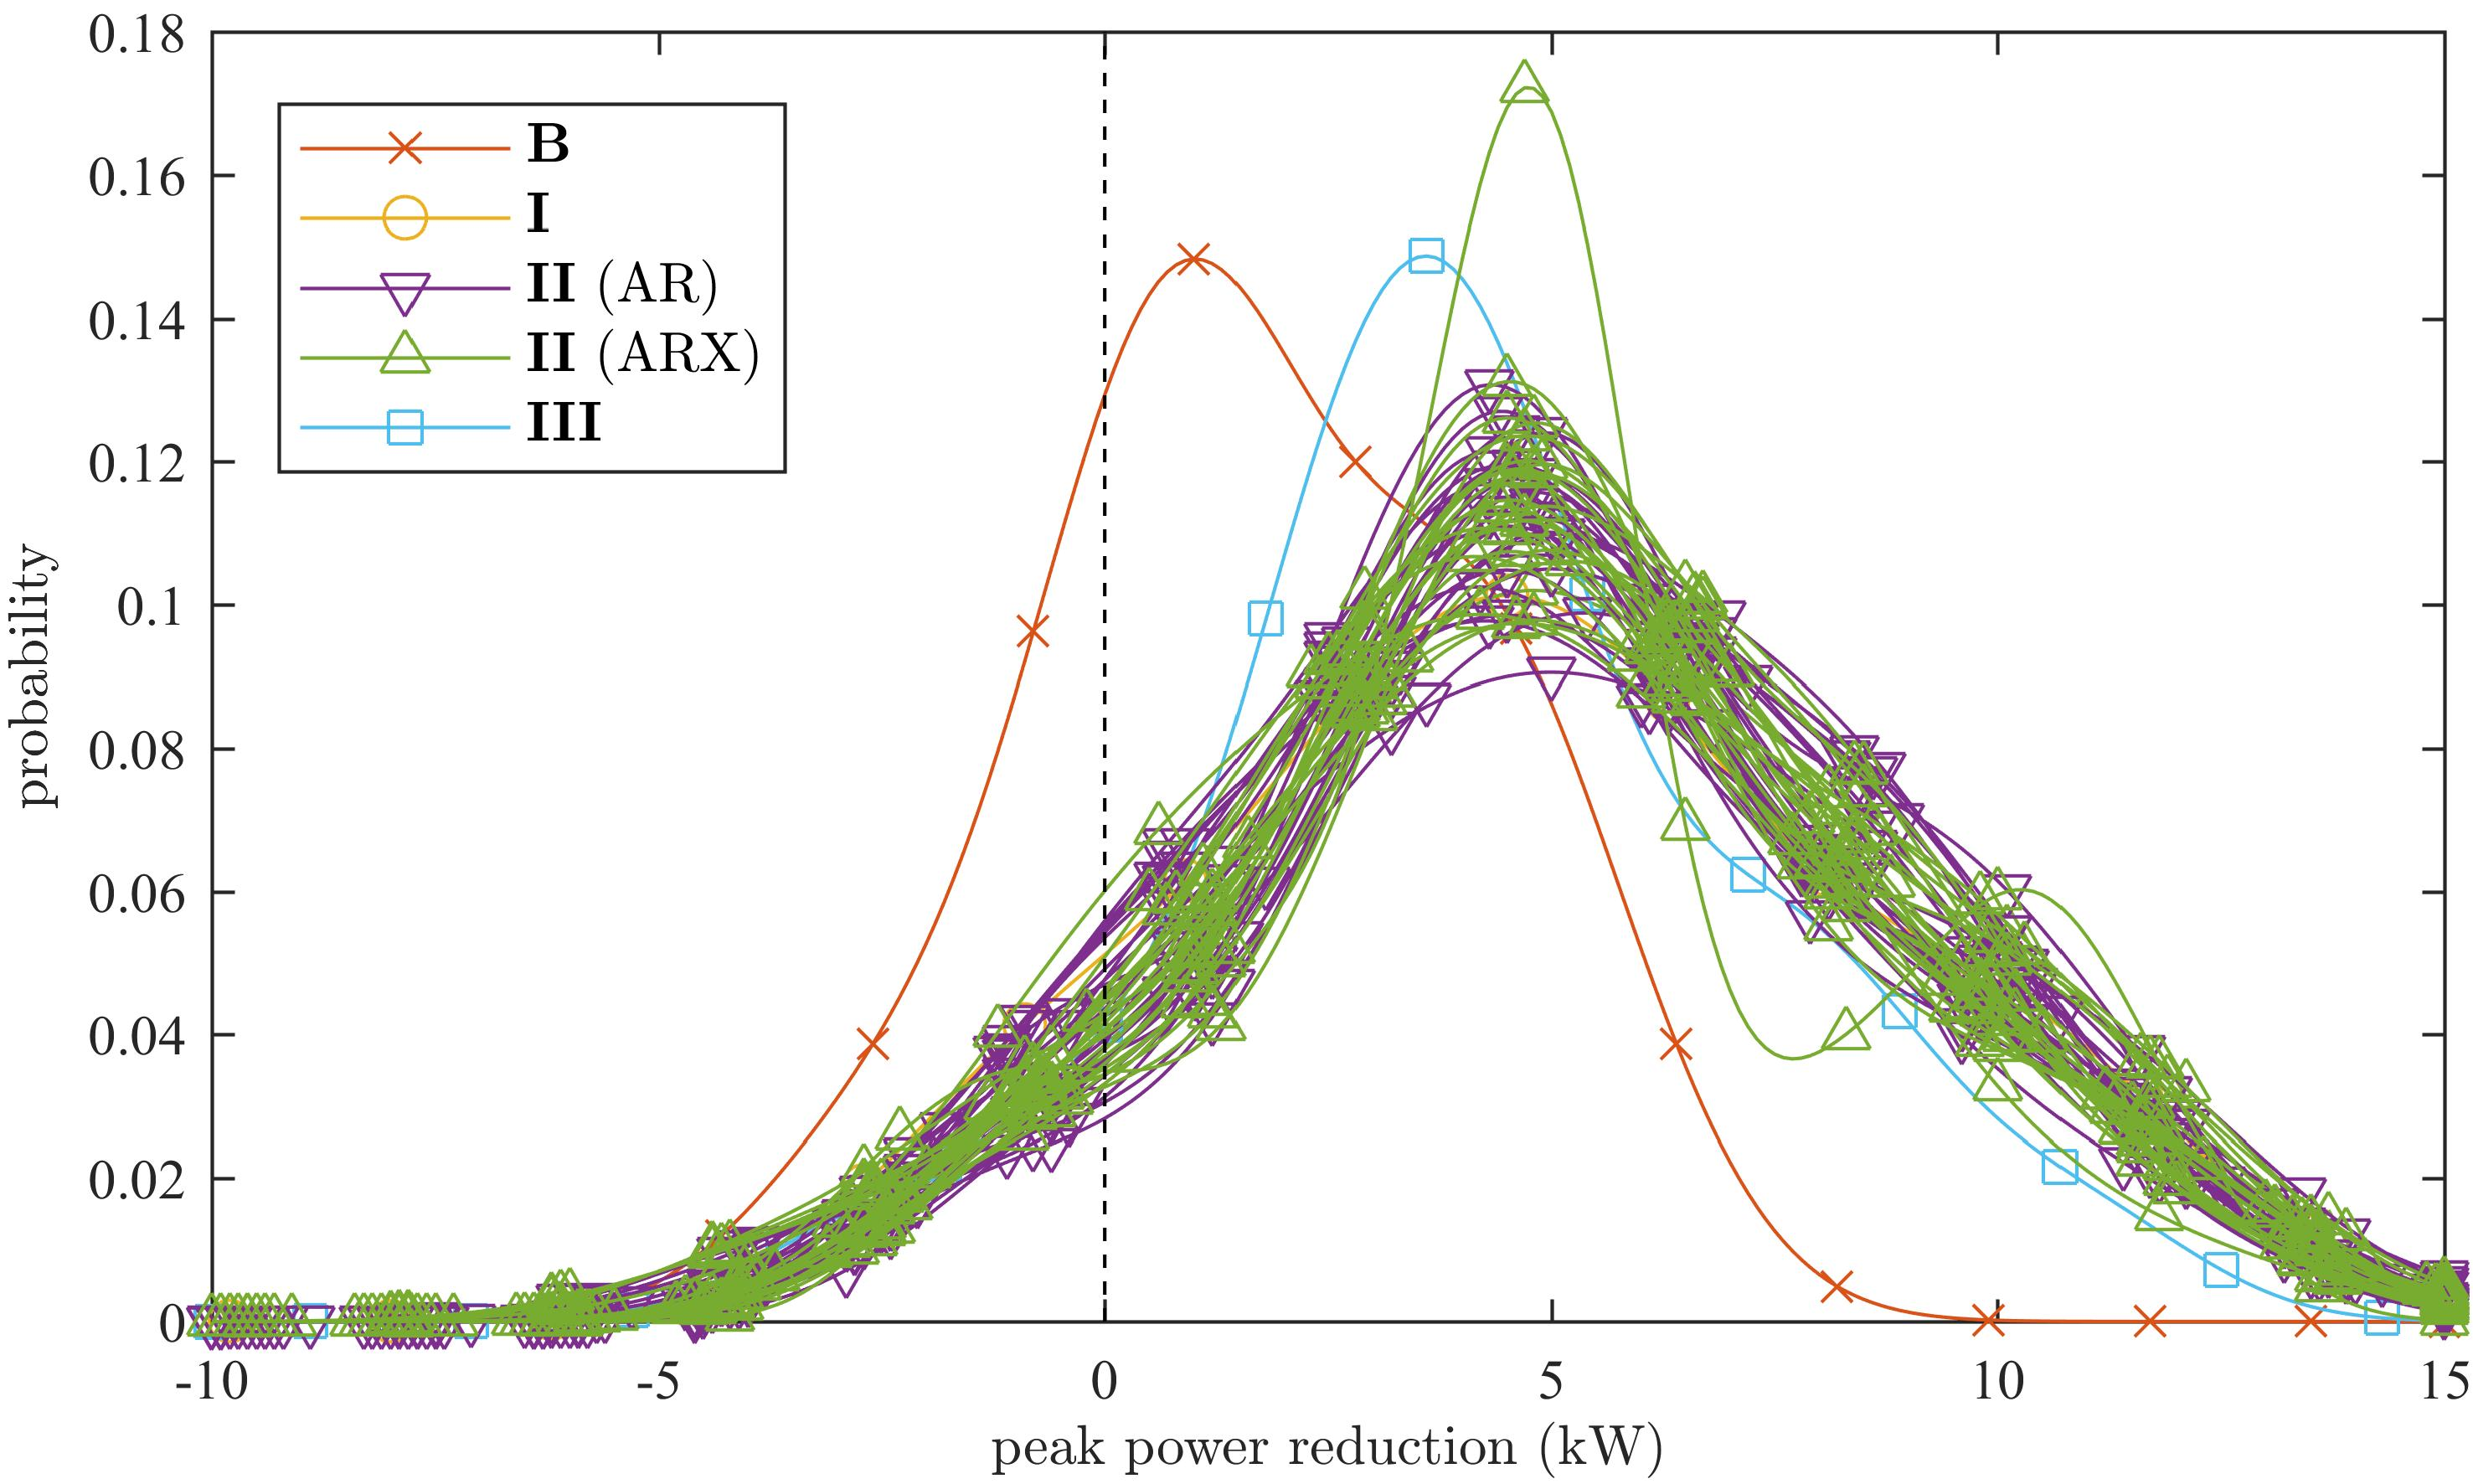
\includegraphics{_chapter2/fig/difference-pdf-1}
%	\subfloat[]{%
%		\includegraphics{_chapter2/fig/pdf-1}
%		\label{ch2:subfig:peak-pdf-1}
%	}
%	\vspace{0mm}
%	\subfloat[]{%
%		\includegraphics{_chapter2/fig/pdf-2}
%		\label{ch2:subfig:peak-pdf-2}
%	}
	\caption{Probability of peak load reduction for different prediction mechanisms and different AR/ARX model lentgths.}
	\label{ch2:fig:peak-pdf-multi-length}
\end{figure}

Similar to Figure~\ref{ch2:fig:peak-diff-pdf}, Figure~\ref{ch2:fig:peak-pdf-multi-length} shows the probability for the difference in peak power between the original case (\textbf{O}) and all other cases.
In this plot however all PDFs for the different model lengths have been included (whilst the previous study only showed the inter-model means).
It can be seen that both the AR and ARX case (i.e. case \textbf{II}) performed noticeably better than the baseline case \textbf{B}.
Despite the varying model length all PDFs appear to peak around a reduction performance of 5kW.
Therefore one may assume that the length of the chosen models does not significantly impact the results.

\begin{figure}\centering
	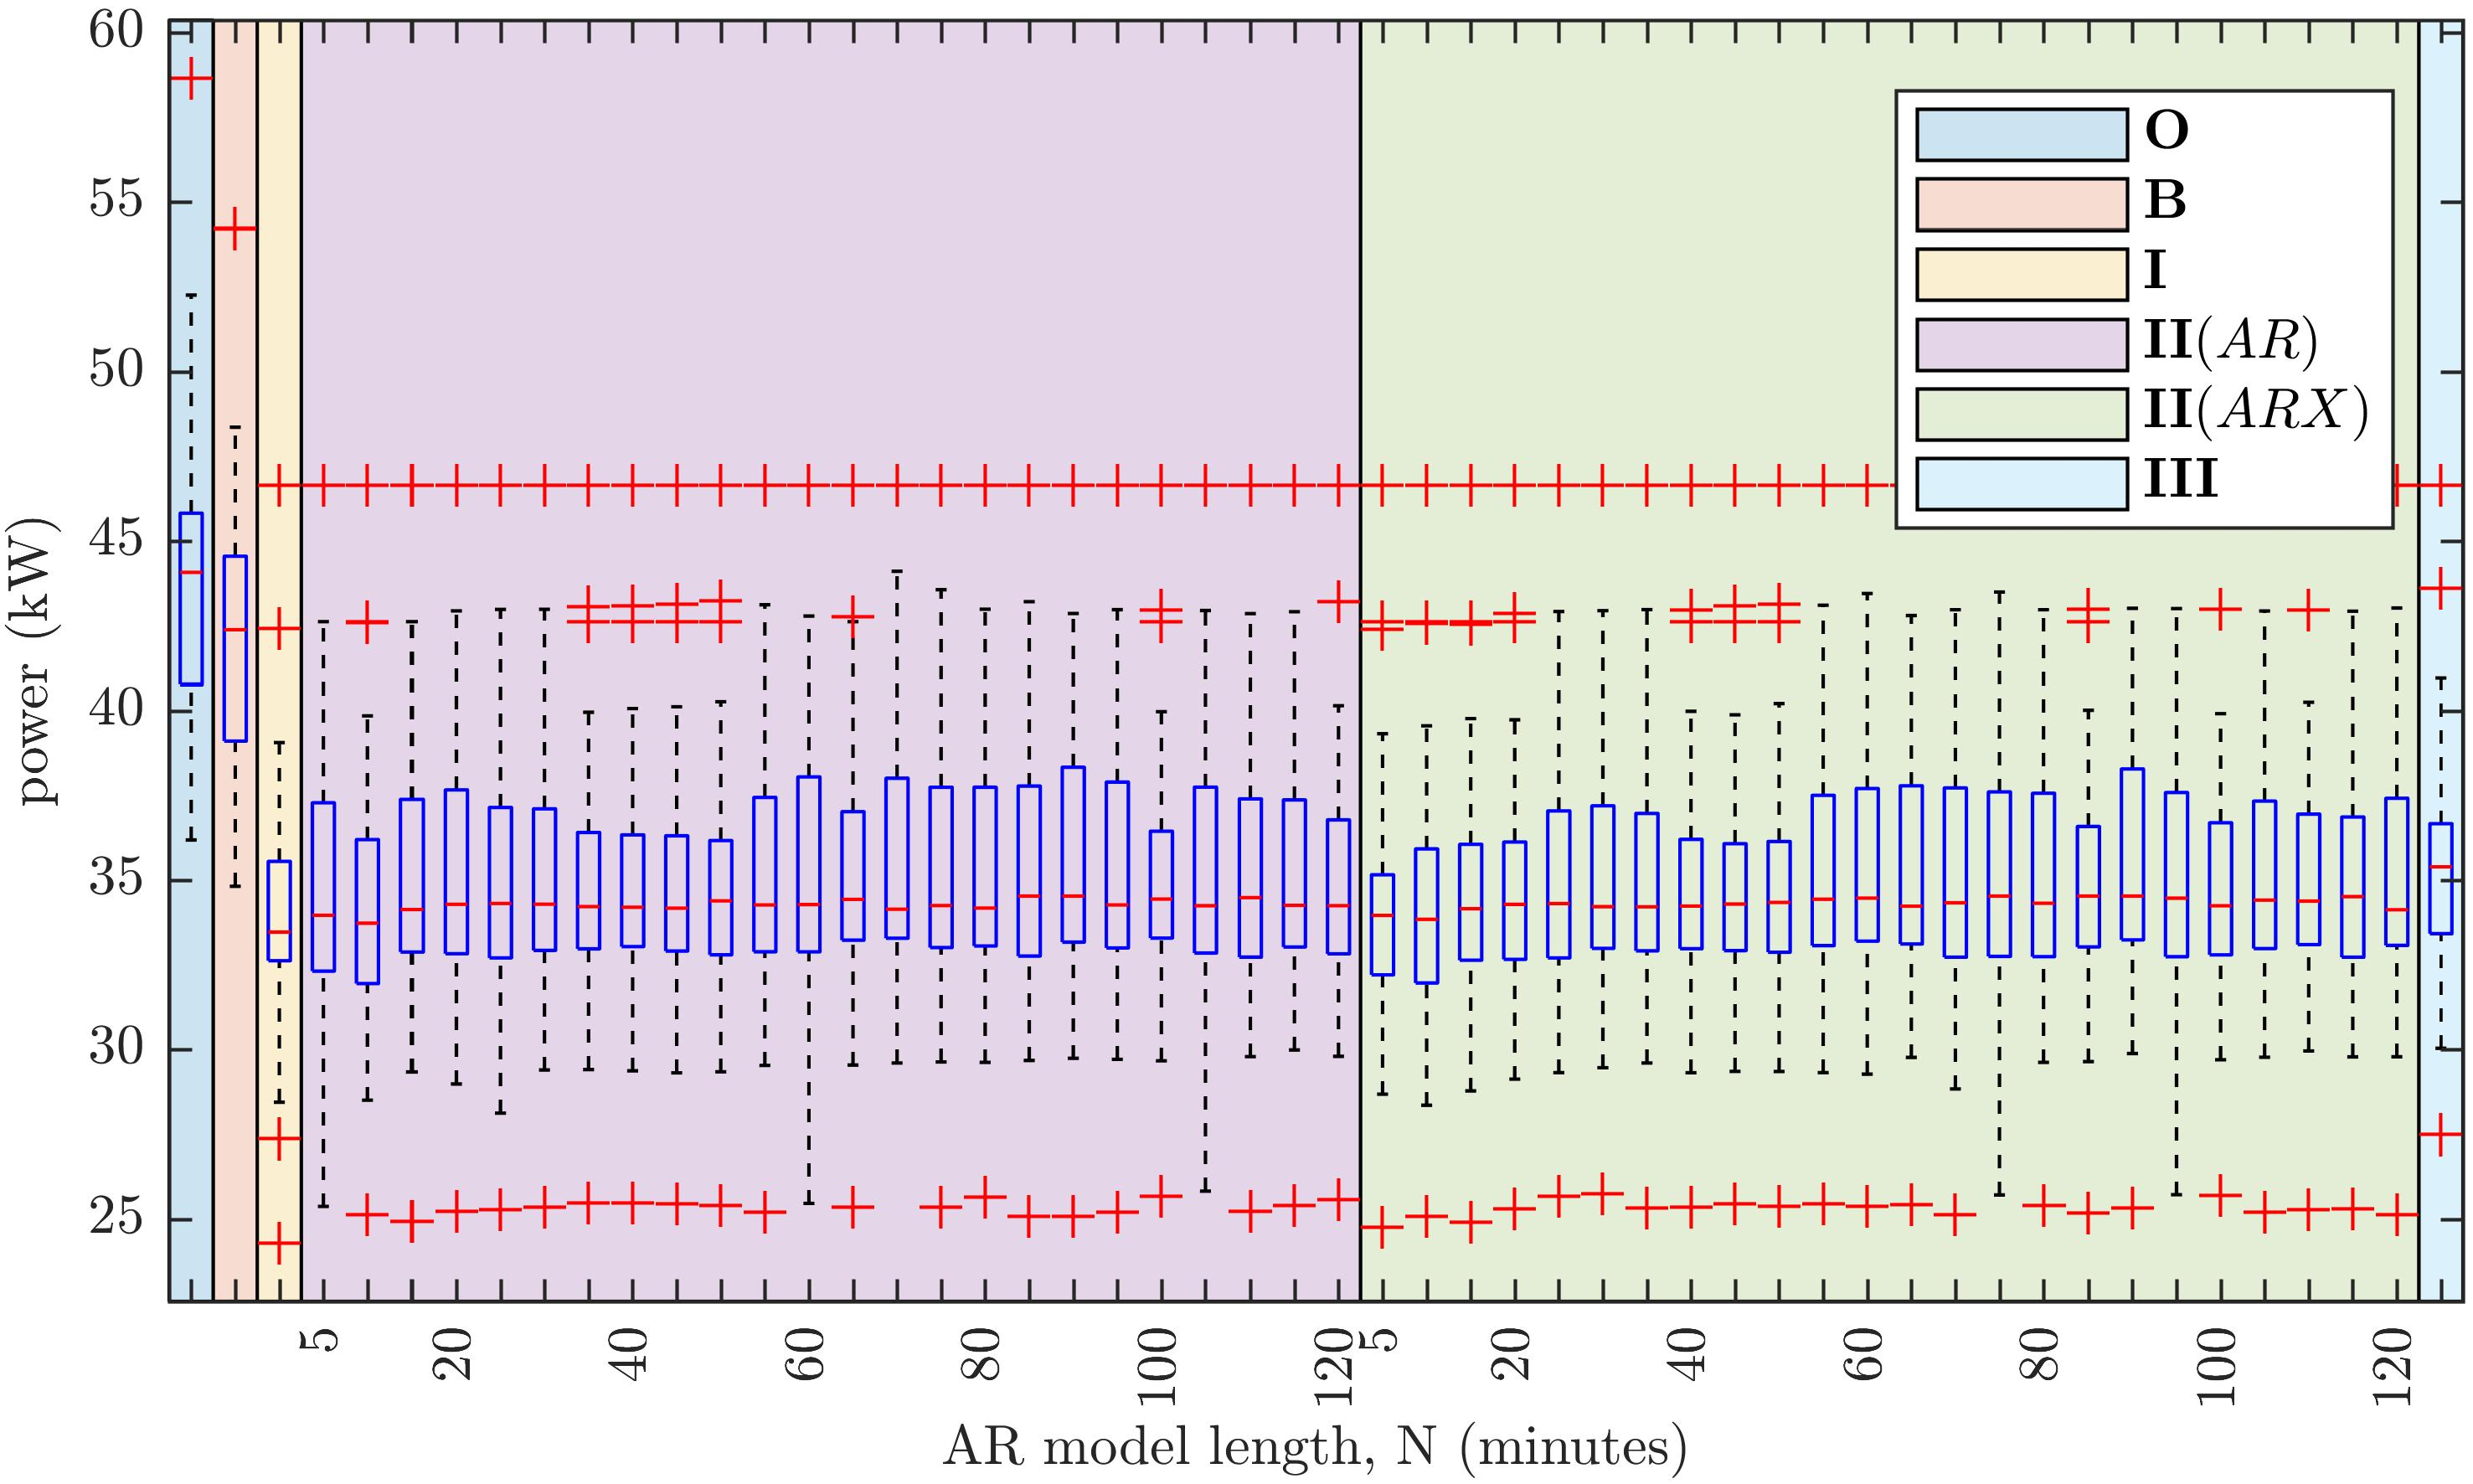
\includegraphics{_chapter2/fig/ar-length-peak-comparison-1}
%	\subfloat[]{%
%		\includegraphics{_chapter2/fig/pdf-1}
%		\label{ch2:subfig:peak-pdf-1}
%	}
%	\vspace{0mm}
%	\subfloat[]{%
%		\includegraphics{_chapter2/fig/pdf-2}
%		\label{ch2:subfig:peak-pdf-2}
%	}
	\caption{Visualisation of the peak power distribution for different AR/ARX model lengths.}
	\label{ch2:fig:boxplot-multi-length}
\end{figure}

This assumption is also supported by the boxplots in Figure~\ref{ch2:fig:boxplot-multi-length} where the peak power distributions are visualised for all different model lengths and the six different case studies.
It can be seen that the different AR/ARX model lengths (i.e. case \textbf{II}) outperforms both the original and baseline cases (i.e. case \textbf{O} and case \textbf{B}, respectively).
All in all, a certain variation in peak reduction performance can be observed, but no apparent trend.
Therefore the assumption that the model length impacts the performance of the dynamic control is true, but for the used data the assumption that a longer model generally yields better results is not.
